\documentclass[11pt, oneside]{article}   	% use "amsart" instead of "article" for AMSLaTeX format
%\usepackage{geometry} 
\usepackage[margin=0.8in]{geometry}                		% See geometry.pdf to learn the layout options. There are lots.
\geometry{letterpaper}                   		% ... or a4paper or a5paper or ... 
%\geometry{landscape}                		% Activate for rotated page geometry
%\usepackage[parfill]{parskip}    		% Activate to begin paragraphs with an empty line rather than an indent
\usepackage{graphicx}				% Use pdf, png, jpg, or eps§ with pdflatex; use eps in DVI mode
								% TeX will automatically convert eps --> pdf in pdflatex		
\usepackage{amsmath}
\usepackage{amssymb}
\usepackage{hyperref}

%SetFonts

%SetFonts
%\vspace{-5ex}

%\title{\vspace{-10ex} Research Proposal: Computational Morality \vspace{-5ex}}
\title{EE958 Competition: Machine Translation System for India}

\author{
    Vasudev Gupta  \\ 
    241562575\\
   {\tt vasudevg24@iitk.ac.in}\\
{Indian Institute of Technology Kanpur (IIT Kanpur)}
}


\date{}							% Activate to display a given date or no date

\begin{document}
\maketitle

% --------------------------------------------------------
% ABSTRACT
% --------------------------------------------------------
\begin{abstract}
This project addresses English-to-Hindi and English-to-Bengali translation for the NLP Capstone competition. I trained Transformer encoder–decoder models with word-level tokenization (30k vocab), using cross-entropy loss, cosine learning rate scheduling, gradient clipping, and checkpointing. The best submission scored chrF++~0.40, ROUGE~0.42, and BLEU~0.14 on the test leaderboard, placing Rank~\#2 overall.  
These results show that carefully tuned Transformer setups can perform strongly on low-resource Indic machine translation. Future improvements could come from subword tokenization (BPE), data augmentation, larger corpora, and exploring decoder-only architectures such as GPT-style models.
\end{abstract}



% --------------------------------------------------------
% COMPETITION RESULT
% --------------------------------------------------------
\section{Competition Result}
\textbf{Codalab Username:} g\_241562575 \\
\textbf{Final leaderboard rank on the test set:} 2 \\
\textbf{chrF++ Score wrt to the final rank:} 0.40 \\
\textbf{ROUGE Score wrt to the final rank:} 0.42 \\
\textbf{BLEU Score wrt to the final rank:} 0.14

% --------------------------------------------------------
% PROBLEM DESCRIPTION
% --------------------------------------------------------
\section{Problem Description}

The project tackles automatic machine translation (MT) from English into two low-resource Indic languages: Hindi and Bengali. MT aims to convert text from a source language into a fluent and semantically accurate target language. The competition provided parallel sentence pairs for English–Hindi and English–Bengali, with systems evaluated on held-out validation and test sets using BLEU, chrF++, and ROUGE.

While large commercial models exist, this task emphasized building systems from scratch with only the provided data. This setup makes the challenge harder but also more instructive: it highlights the core objectives, design trade-offs, and difficulties of training translation models without relying on massive pretraining.

% --------------------------------------------------------
% DATA ANALYSIS
% --------------------------------------------------------

\section{Data Analysis}

\subsection{Dataset Overview}
The competition datasets cover English$\rightarrow$Bengali and English$\rightarrow$Hindi, each split into train, validation, and test sets. Target translations for validation and test are withheld for scoring, so summary statistics are available only on training data.

\subsection{Corpus Statistics}
Tables~\ref{tab:bengali_stats} and \ref{tab:hindi_stats} summarize basic length statistics (in words, approximately) for source and target sides.

\begin{table}[h]
\centering
\caption{English$\rightarrow$Bengali corpus statistics (lengths in words).}
\label{tab:bengali_stats}
\begin{tabular}{|l|c|c|c|c|c|c|}
\hline
\textbf{Split} & \textbf{count} & \textbf{source\_mean} & \textbf{source\_min} & \textbf{source\_max} & \textbf{target\_mean} & \textbf{target\_min / max} \\
\hline
Train       & 68{,}849 & 16.82 & 1.0 & 100.0 & 14.27 & 1.0 / 84.0 \\
Validation  & 9{,}836  & 16.88 & 1.0 & 175.0 & --    & -- \\
Test        & 19{,}672 & 16.93 & 0.0 & 99.0  & --    & -- \\
\hline
\end{tabular}
\end{table}

\begin{table}[h]
\centering
\caption{English$\rightarrow$Hindi corpus statistics (lengths in words).}
\label{tab:hindi_stats}
\begin{tabular}{|l|c|c|c|c|c|c|}
\hline
\textbf{Split} & \textbf{count} & \textbf{source\_mean} & \textbf{source\_min} & \textbf{source\_max} & \textbf{target\_mean} & \textbf{target\_min / max} \\
\hline
Train       & 80{,}797 & 17.07 & 1.0 & 257.0 & 18.93 & 1.0 / 216.0 \\
Validation  & 11{,}543 & 17.08 & 1.0 & 128.0 & --    & -- \\
Test        & 23{,}085 & 17.08 & 1.0 & 155.0 & --    & -- \\
\hline
\end{tabular}
\end{table}

\subsection{Length Distributions}
Figure~\ref{fig:kde_plots} shows KDE plots of sentence-length distributions (train/val/test) for both translation tasks. The source-side distributions are well aligned across splits (means $\approx$ 17 words), indicating consistent difficulty between train and evaluation data.

\begin{figure}[h]
    \centering
    \begin{minipage}{0.48\textwidth}
        \centering
        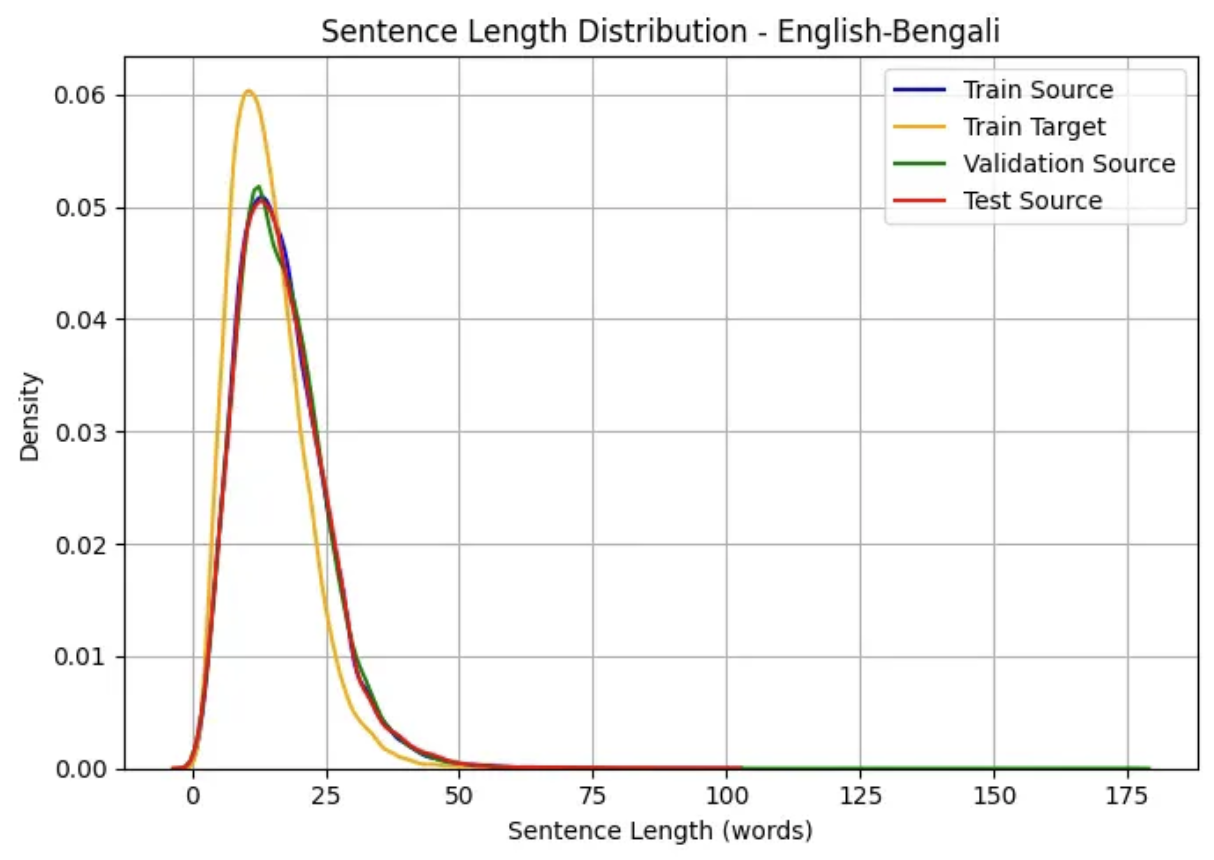
\includegraphics[width=\linewidth]{eda/engbengali_stats.png}
        \label{fig:engbengali_kde}
    \end{minipage}\hfill
    \begin{minipage}{0.48\textwidth}
        \centering
        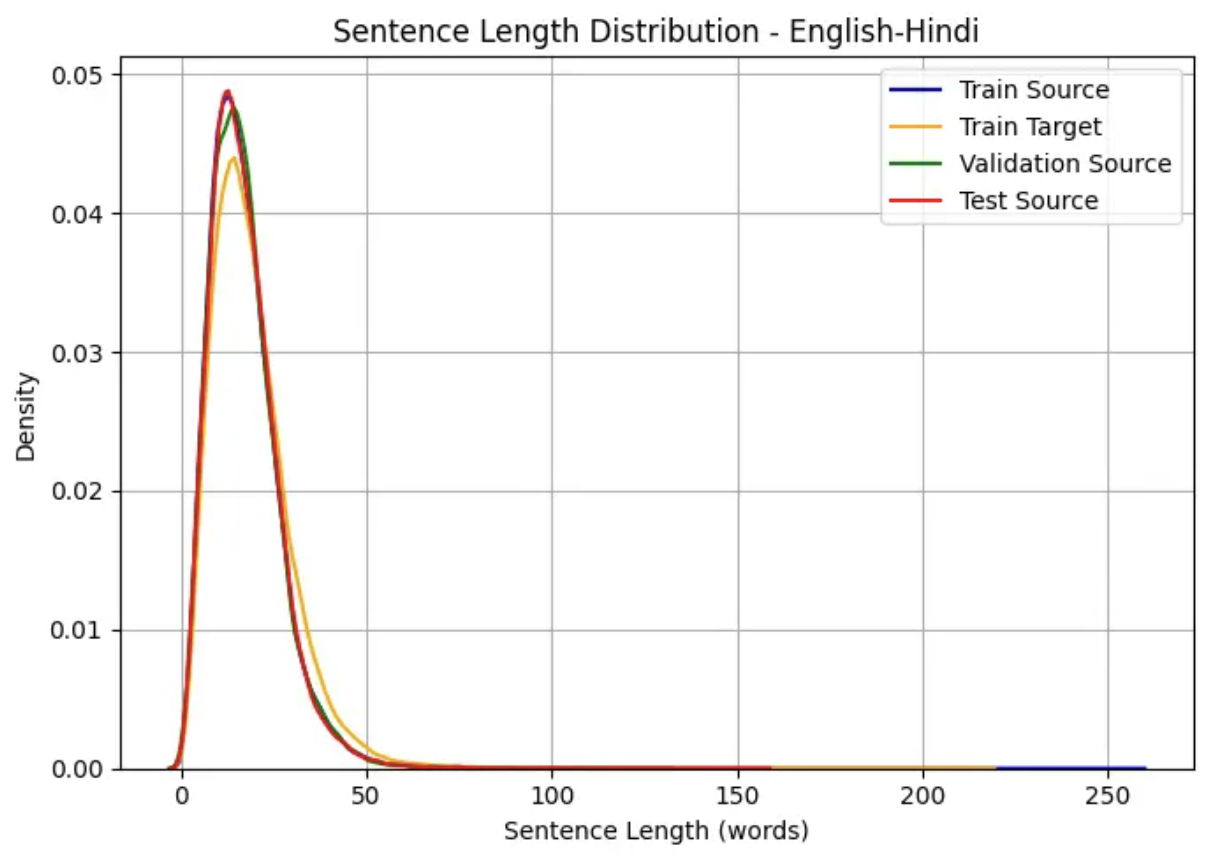
\includegraphics[width=\linewidth]{eda/enghindi_stats.png}
        \label{fig:enghindi_kde}
    \end{minipage}
    \caption{Sentence length distributions (train/val/test) for English$\rightarrow$Bengali (left) and English$\rightarrow$Hindi (right).}
    \label{fig:kde_plots}
\end{figure}

\subsection{Key Observations}
\begin{itemize}
    \item Source lengths are stable across splits ($\sim$17 words), indicating little covariate shift.  
    \item Hindi targets are longer on average (18.9 vs.\ 14.3 for Bengali), reflecting richer morphology.  
    \item Both corpora contain long-tail sentences (up to 257 tokens), so training capped sequences at 256 tokens for efficiency.  
    \item Validation/test target stats are hidden, but aligned source distributions reduce evaluation mismatch.  
\end{itemize}

% --------------------------------------------------------
% MODEL DESCRIPTION
% --------------------------------------------------------
 \section{Model Description}
\subsection{Model Evolution}
The approach was based on the Transformer encoder–decoder architecture \cite{vaswani2017attention}. I first implemented it from scratch in PyTorch, which was slow and unstable, then switched to PyTorch’s optimized \texttt{nn.Transformer} \cite{paszke2019pytorch,pytorchdocs} for faster, more stable training.  
I also tried subword tokenization with BPE \cite{sennrich2016neural} and SentencePiece \cite{kudo2018sentencepiece}, though my best submissions used word-level vocabularies. Decoder-only GPT-style models were partly explored \cite{radford2019language,brown2020language}, but not fully completed in time.


\subsection{Final Model}
Both English-to-Hindi and English-to-Bengali systems used a Transformer encoder–decoder with word-level tokenization (30k vocab, max length 256). The main hyperparameters were:

\begin{itemize}
    \item \textbf{English-to-Hindi:} $d_{model}=128$, $n_{heads}=8$, $n_{layers}=6$, $d_{ff}=512$, dropout $=0.1$, batch size $=32$, 30 epochs. Learning rate peaked at $9\times10^{-4}$ with cosine decay, final LR $9\times10^{-5}$, and 3.5\% warmup.  
    \item \textbf{English-to-Bengali:} Same architecture, but $n_{heads}=4$ and peak LR $6\times10^{-4}$ (final $6\times10^{-5}$).  
\end{itemize}

Training progress was tracked in Weights \& Biases (wandb), and checkpoints were saved regularly.

\subsection{Objective Function}
Training used token-level cross-entropy loss, implemented with PyTorch \cite{paszke2019pytorch,pytorchdocs}. For each target token $y_t$,
\[
\mathcal{L}(\theta) = - \sum_{t=1}^{T} m_t \, \log p_\theta(y_t \mid y_{<t}, x),
\]
where $x$ is the source sentence and $m_t$ masks out PAD tokens.


\subsection{Inference Strategy}
Inference used greedy decoding: at each step, the token with highest probability was chosen until an end-of-sequence token or maximum length was reached. While beam search may yield higher scores, greedy decoding was sufficient for leaderboard submissions.


% --------------------------------------------------------
% EXPERIMENTS
% --------------------------------------------------------
\section{Experiments}

\subsection{Data Pre-Processing}

\subsubsection{Data Format}  
The raw dataset was provided in JSON. For efficient streaming during training, I converted it into JSONL, where each line contains one source–target pair. This avoided loading the entire dataset into memory.

\subsubsection{Tokenization}  
English text was lowercased, whitespace-normalized, and split on punctuation. A 30k word-level vocabulary was built with four special tokens: \texttt{<PAD>}, \texttt{<UNK>}, \texttt{<SOS>}, \texttt{<EOS>}. Hindi and Bengali text used regex patterns from the Indic NLP Library \cite{indicnlp} to handle script-specific punctuation and numerals.



A simplified version of my tokenizer logic:  
\begin{verbatim}
def text_to_sequence(text, word2idx, max_len):
    tokens = tokenize(text)
    seq = [word2idx["<SOS>"]]
    for tok in tokens:
        if len(seq) >= max_len - 1: break
        seq.append(word2idx.get(tok, word2idx["<UNK>"]))
    seq.append(word2idx["<EOS>"])
    return pad(seq, max_len, word2idx["<PAD>"])
\end{verbatim}

\subsubsection{Data Loader}  
I wrote a minimal custom loader (\texttt{DataLoaderLite}) to cycle through batches sequentially, rather than PyTorch’s heavier \texttt{DataLoader}. This made training loops transparent and easy to debug.

\begin{verbatim}
class DataLoaderLite:
    def __init__(self, X, y, batch_size):
        self.X, self.y, self.bs = X, y, batch_size
        self.i, self.epoch = 0, 0

    def next_batch(self):
        start, end = self.i, self.i + self.bs
        if end > len(self.X):  # restart epoch
            self.epoch += 1
            start, end, self.i = 0, self.bs, self.bs
        else:
            self.i = end
        return self.X[start:end], self.y[start:end]
\end{verbatim}

\subsection{Training Procedure}

\subsubsection{Optimizer and Schedule}  
Models were trained with AdamW \cite{loshchilov2019decoupled} (extending Adam \cite{kingma2015adam}) and gradient clipping. The learning rate followed a cosine decay schedule with warm restarts \cite{loshchilov2016sgdr}, with 3.5\% warmup.



\begin{verbatim}
if step < warmup_steps:
    lr = max_lr * (step+1)/warmup_steps
else:
    decay = (step - warmup_steps) / (MAX - warmup_steps)
    coeff = 0.5 * (1 + cos(pi * decay))
    lr = min_lr + coeff * (max_lr - min_lr)
\end{verbatim}

Peak LR was task-specific: $9\times10^{-4}$ for Hindi, $6\times10^{-4}$ for Bengali.  
Figure~\ref{fig:lrshape} shows the curve over 30k steps.

\begin{figure}[h]
    \centering
    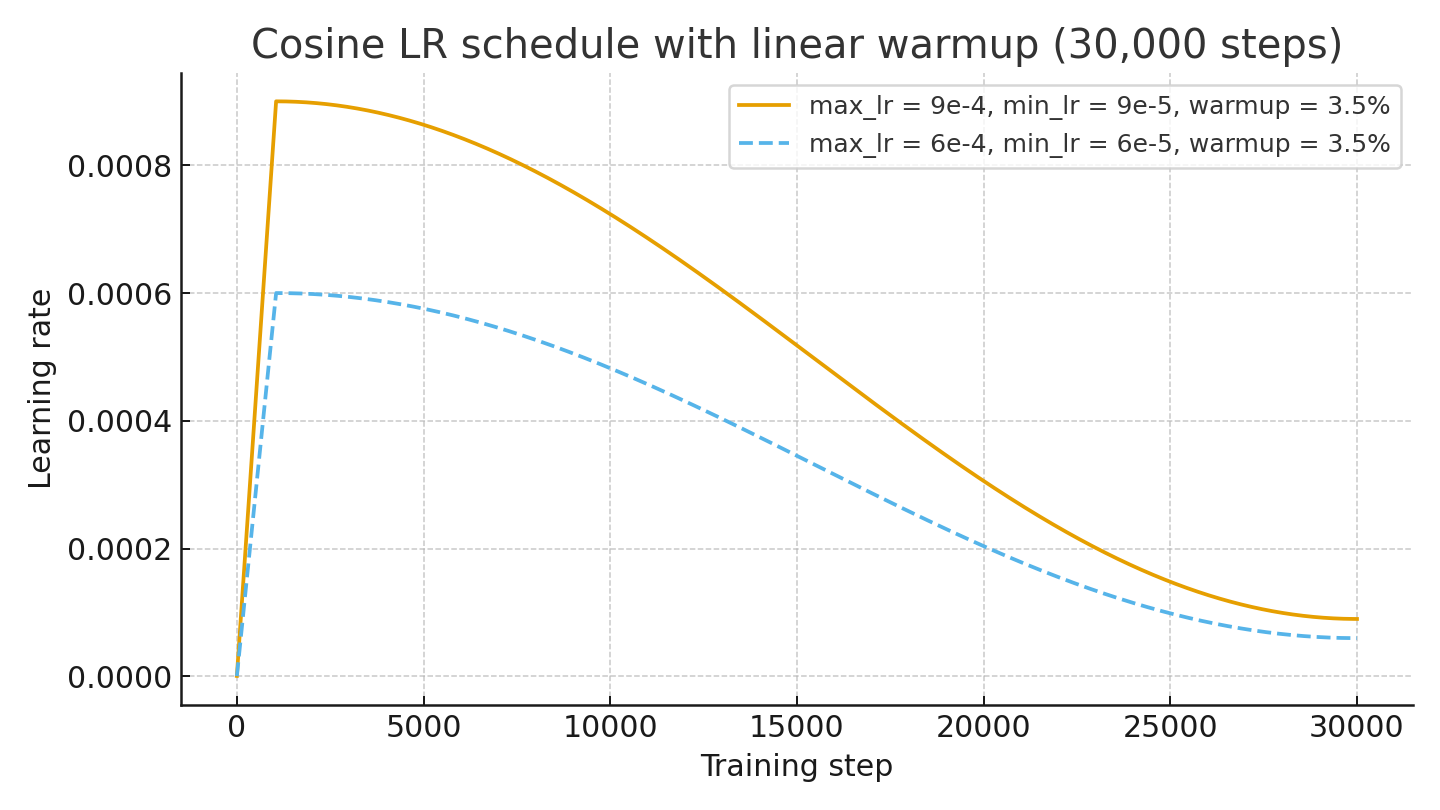
\includegraphics[width=0.75\linewidth]{eda/lr_schedule_30k.png}
    \caption{Cosine learning rate schedule with 3.5\% warmup over 30,000 steps.}
    \label{fig:lrshape}
\end{figure}

\subsubsection{Main Experiment Configurations}  
Three main experiments were run, progressively refining implementation and hyperparameters. Table~\ref{tab:experiment_configs} summarizes the setups.

\begin{table}[h]
\centering
\caption{Main Experiment Configurations}
\label{tab:experiment_configs}
\resizebox{\textwidth}{!}{%
\begin{tabular}{|l|c|c|c|}
\hline
\textbf{Configuration} & \textbf{Experiment 1 (exp3)} & \textbf{Experiment 2 (exp4)} & \textbf{Experiment 3 (exp4.1)} \\
\hline
Implementation & Custom Transformer & PyTorch nn.Transformer & PyTorch nn.Transformer \\
$d_{model}$ & 128 & 128 & 128 \\
$n_{layers}$ & 6 & 6 & 6 \\
$d_{ff}$ & 512 & 512 & 512 \\
$n_{heads}$ (Hindi) & 4 & 4 & 8 \\
$n_{heads}$ (Bengali) & 4 & 4 & 4 \\
Epochs & 10 & 10 & 30 \\
Batch Size & 32 & 32 & 32 \\
Vocab Size & 30k & 30k & 30k \\
Peak LR (Hindi) & $6\!\times\!10^{-4}$ & $6\!\times\!10^{-4}$ & $9\!\times\!10^{-4}$ \\
Peak LR (Bengali) & $6\!\times\!10^{-4}$ & $6\!\times\!10^{-4}$ & $6\!\times\!10^{-4}$ \\
Schedule & Cosine & Cosine & Cosine \\
\hline
\end{tabular}%
}
\end{table}

\subsubsection{Training Dynamics}  
Figures~\ref{fig:loss_hindi}--\ref{fig:gpu_bengali} illustrate training curves for both language pairs, including loss, validation, learning rate, gradient norms, and GPU dynamics (Multiprocessing clock speed). The custom Transformer showed unstable GPU usage (\ref{fig:gpu_hindi}, \ref{fig:gpu_bengali}), highlighting inefficiencies compared to the PyTorch implementation. Gradient norms were expected to remain stable but instead grew over time, which was a concern during training. Loss curves (train and validation) improved steadily, though Experiment~3 eventually began to overfit after extended training.


\begin{figure}[h]
\centering
\begin{minipage}{0.18\textwidth}
    \centering
    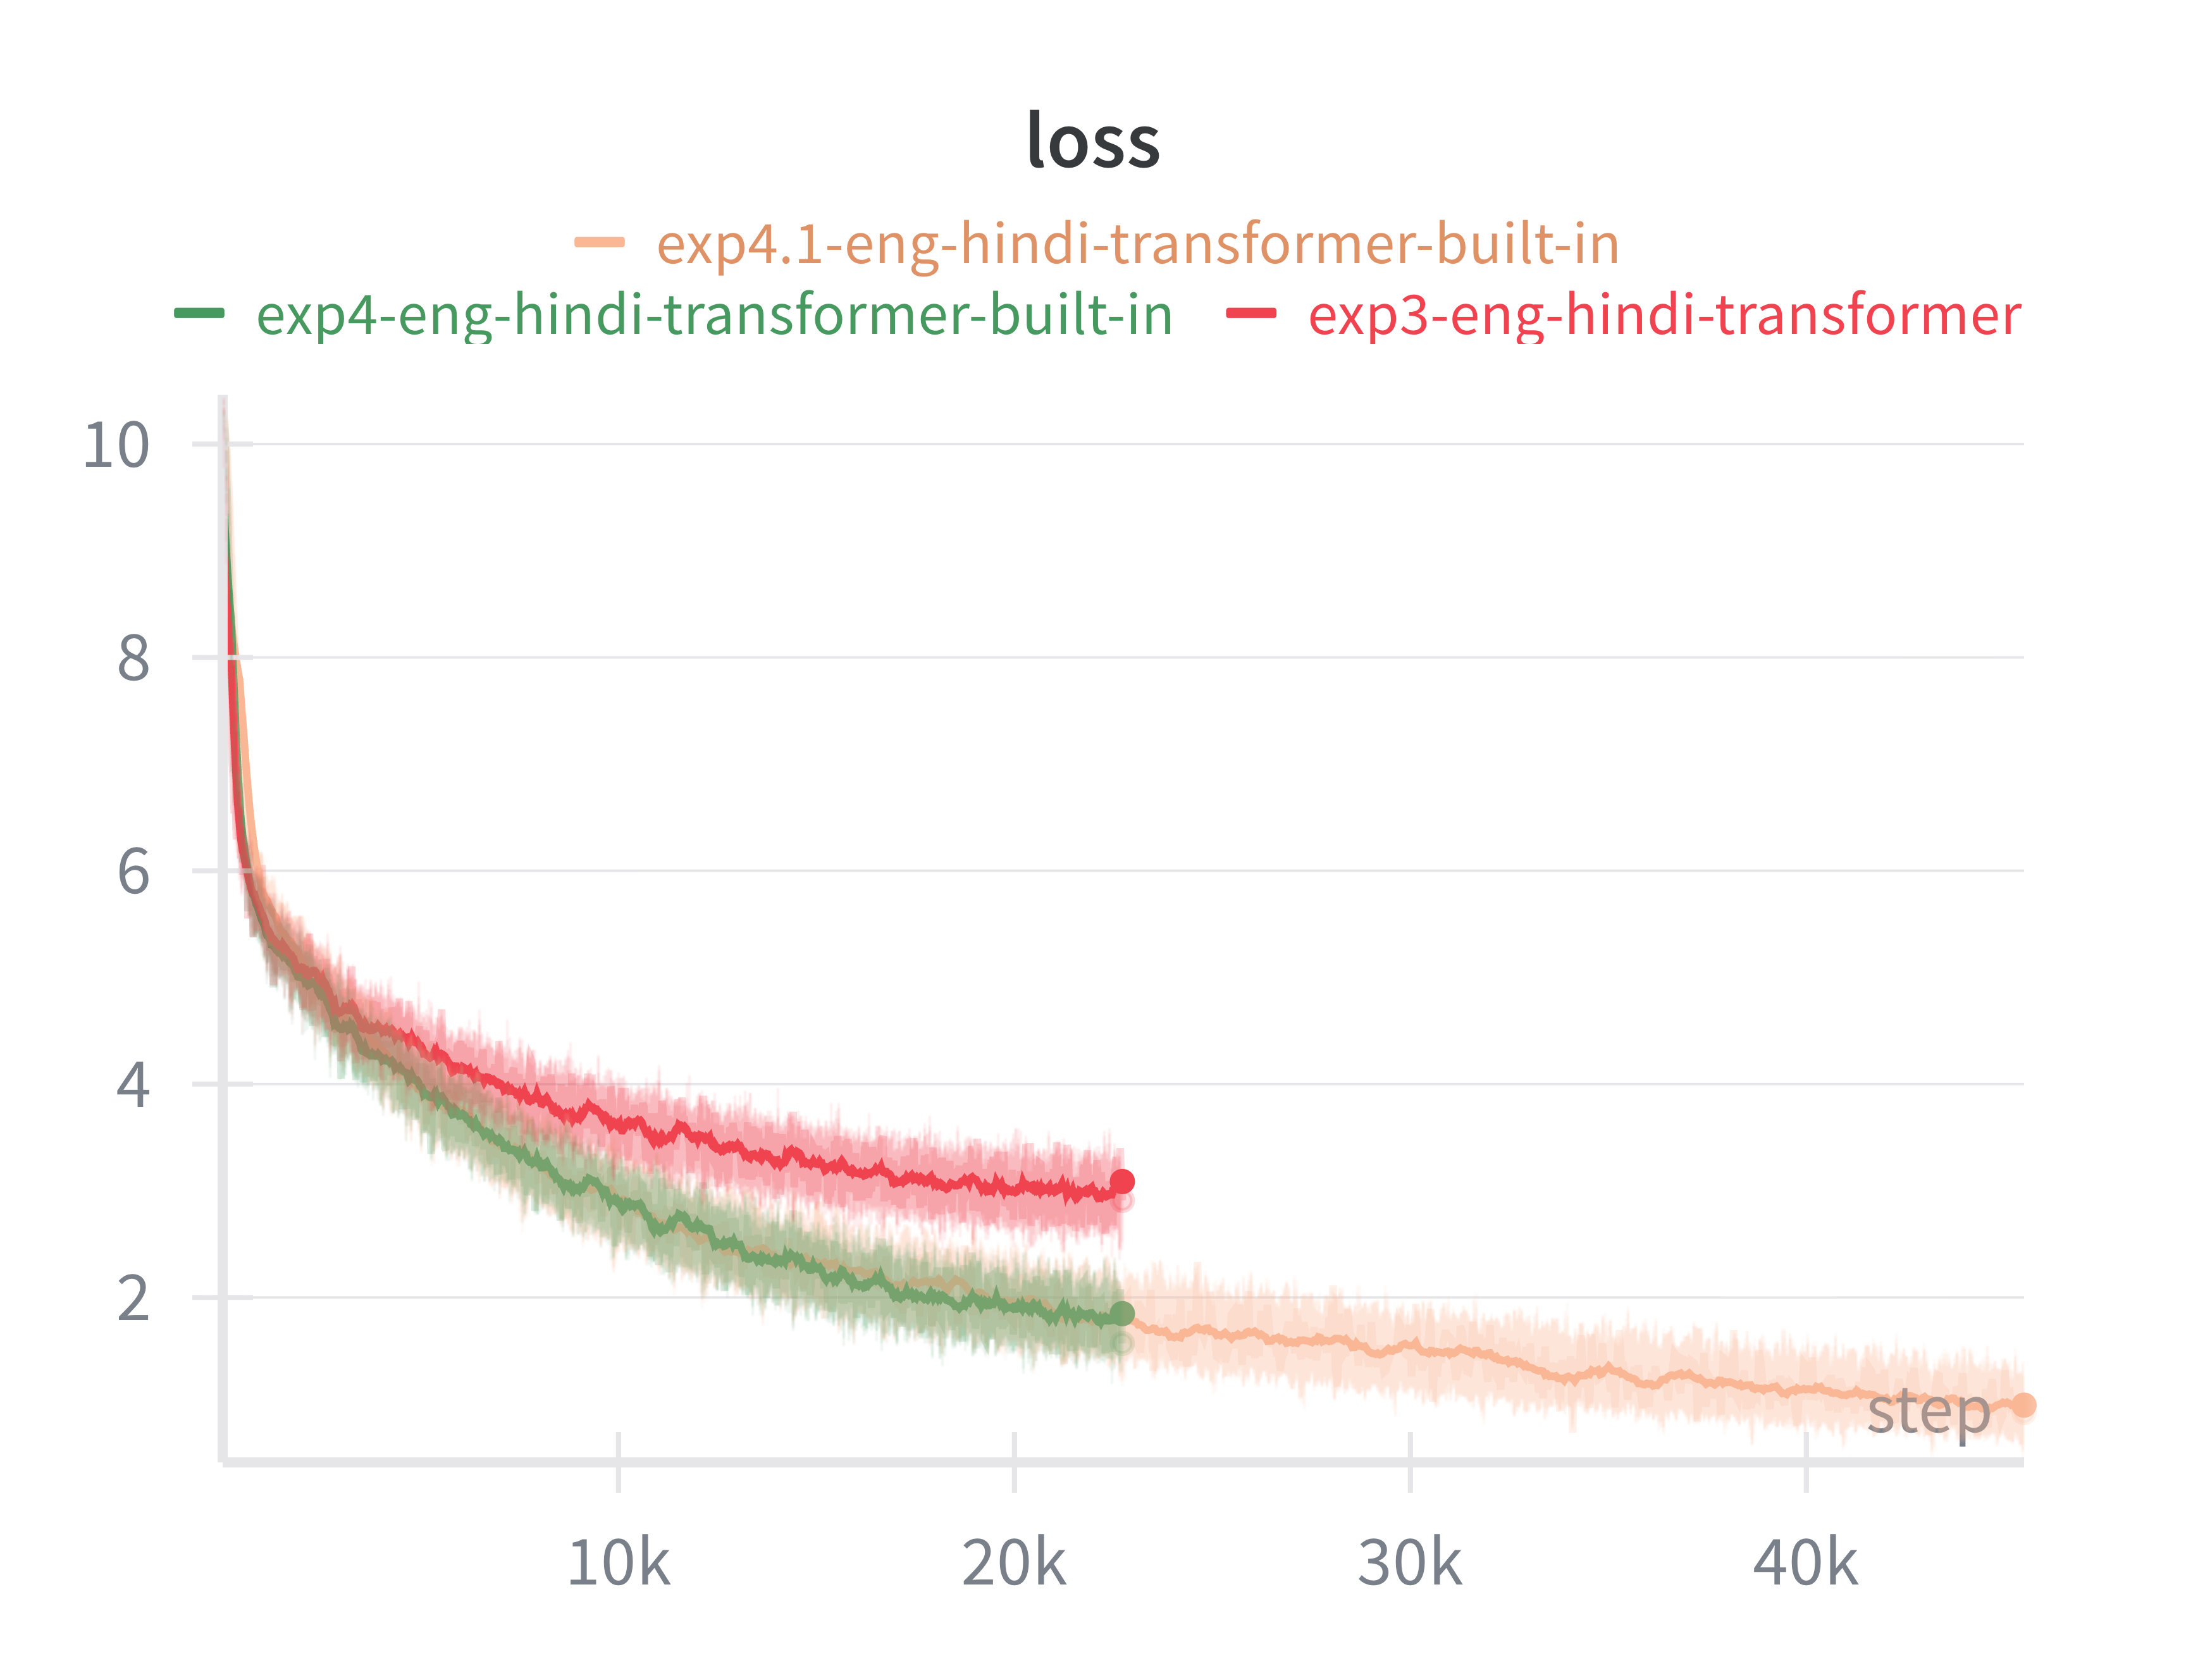
\includegraphics[width=\textwidth]{wandb/cross_entropy_loss_hindi.png}
    \caption{Training loss (Hindi)}
    \label{fig:loss_hindi}
\end{minipage}
\hfill
\begin{minipage}{0.18\textwidth}
    \centering
    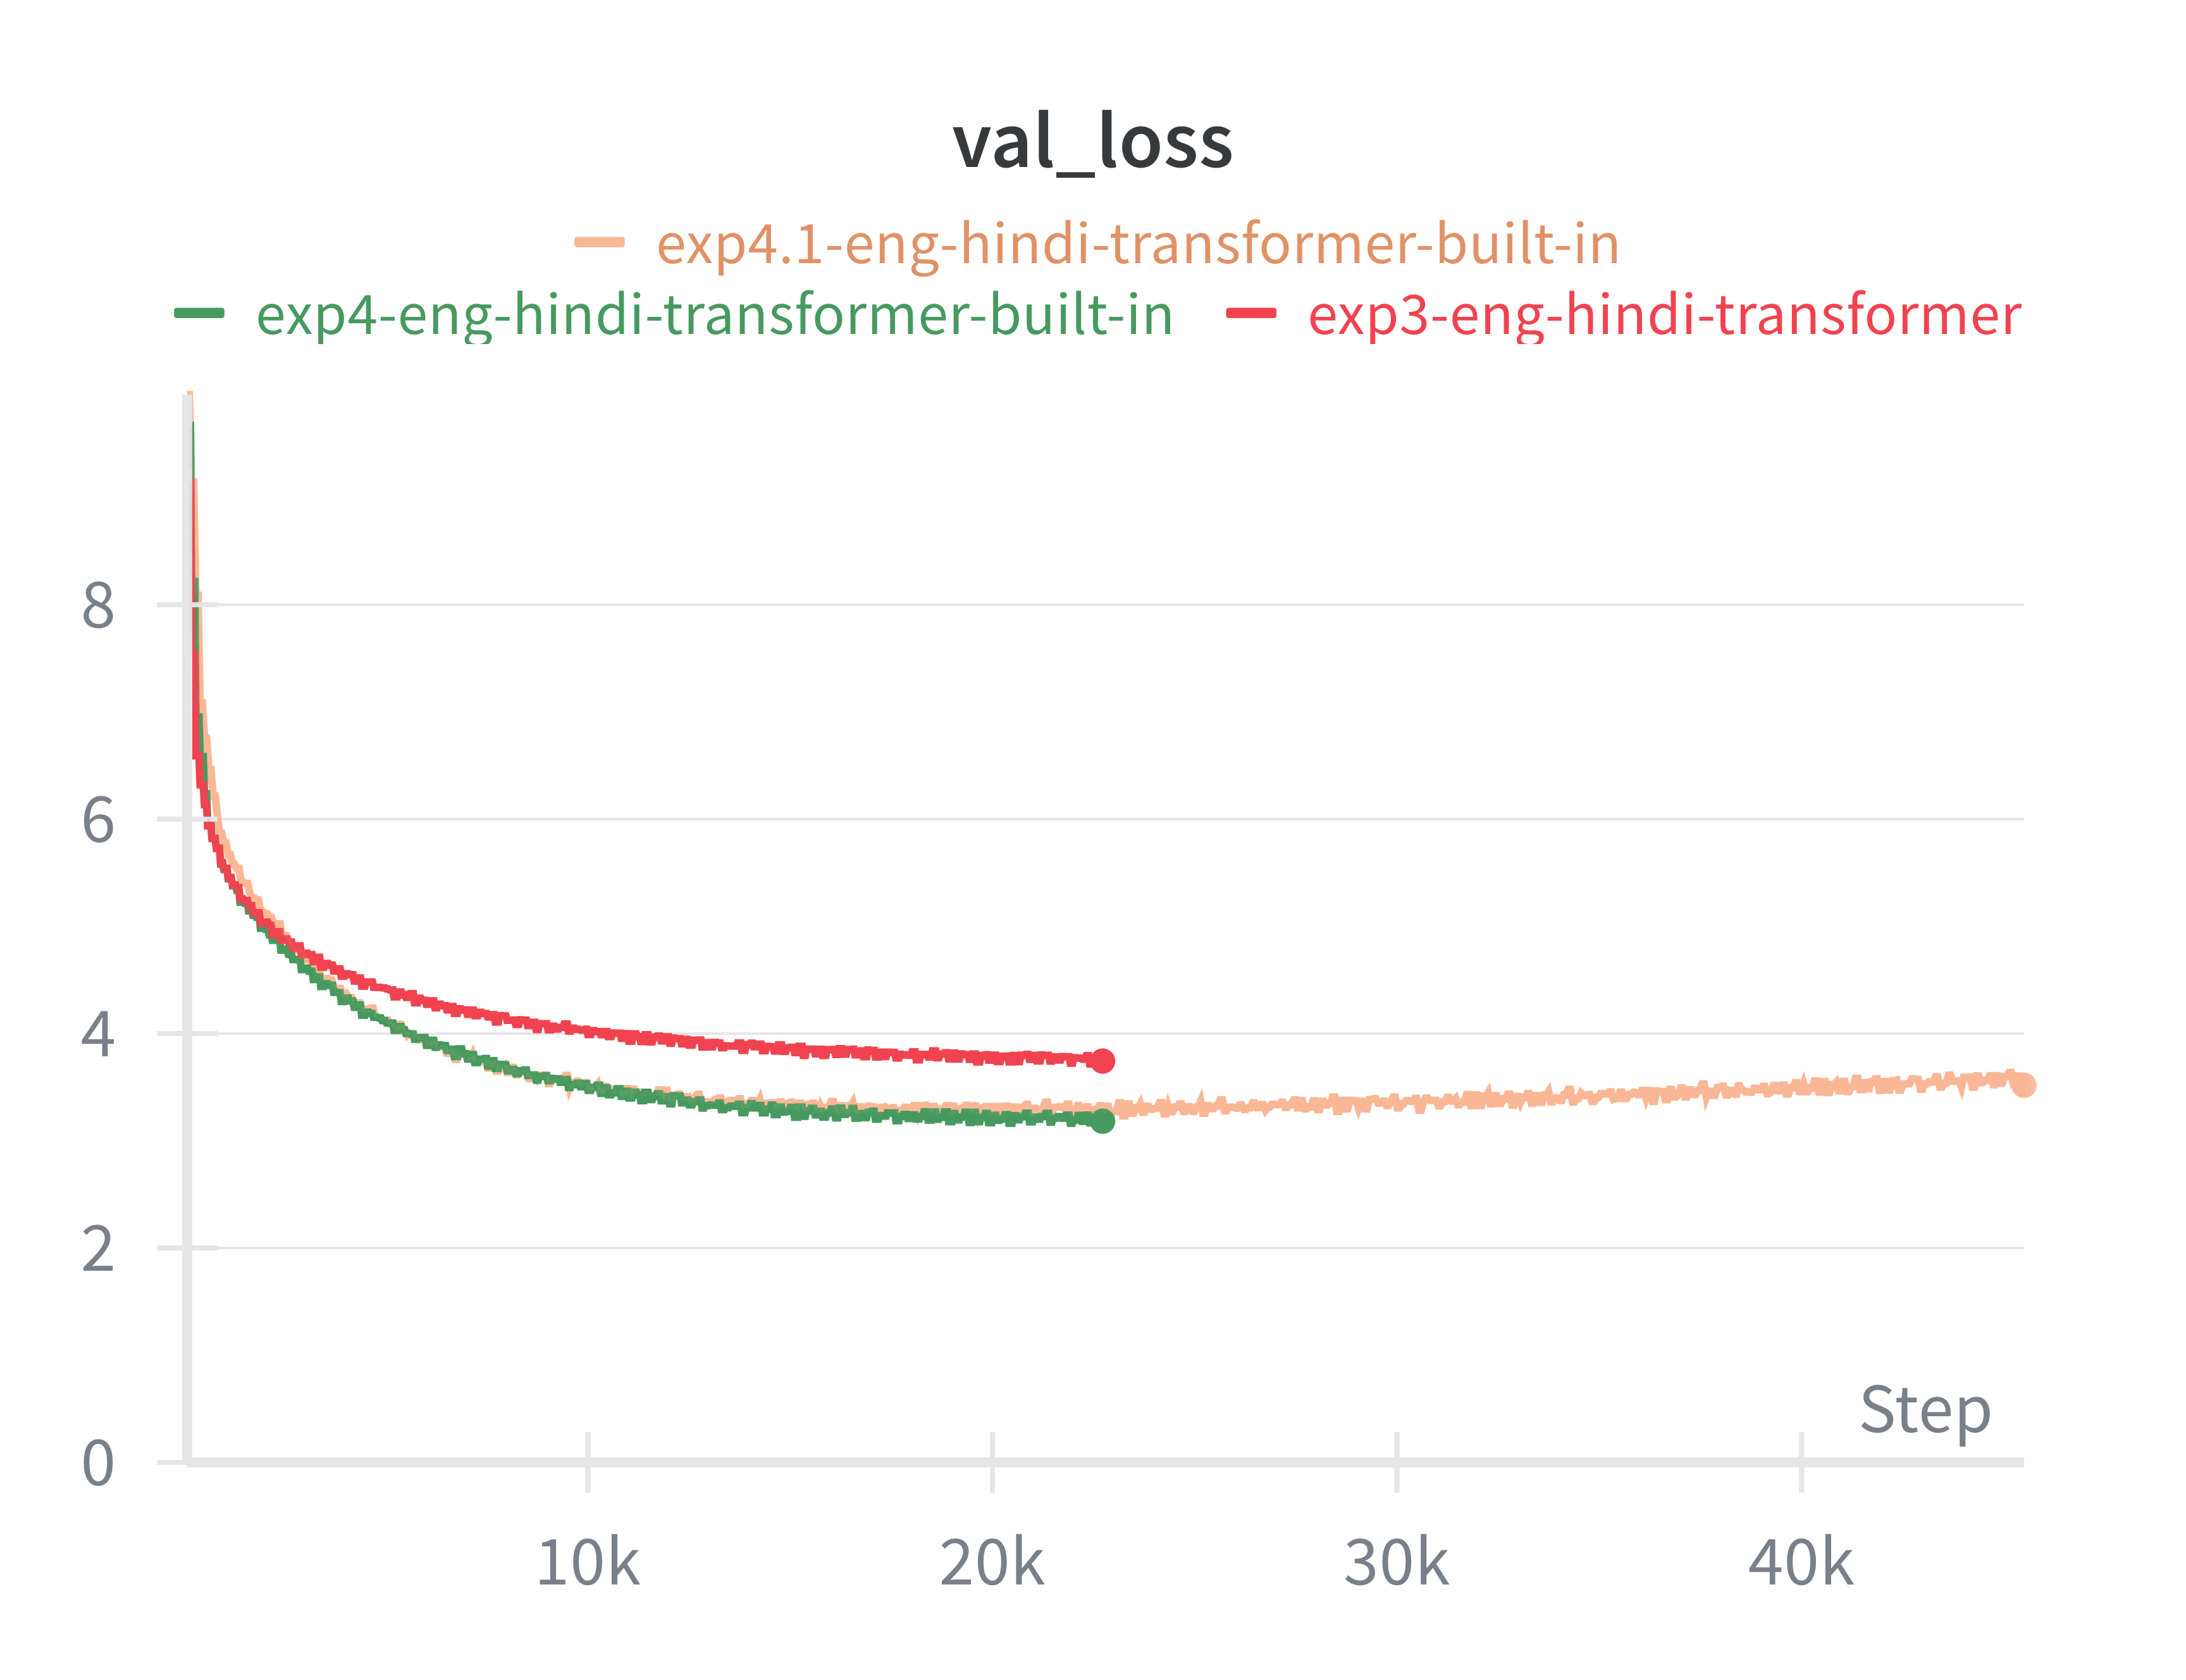
\includegraphics[width=\textwidth]{wandb/val_loss_hindi.png}
    \caption{Validation loss (Hindi)}
    \label{fig:val_loss_hindi}
\end{minipage}
\hfill
\begin{minipage}{0.18\textwidth}
    \centering
    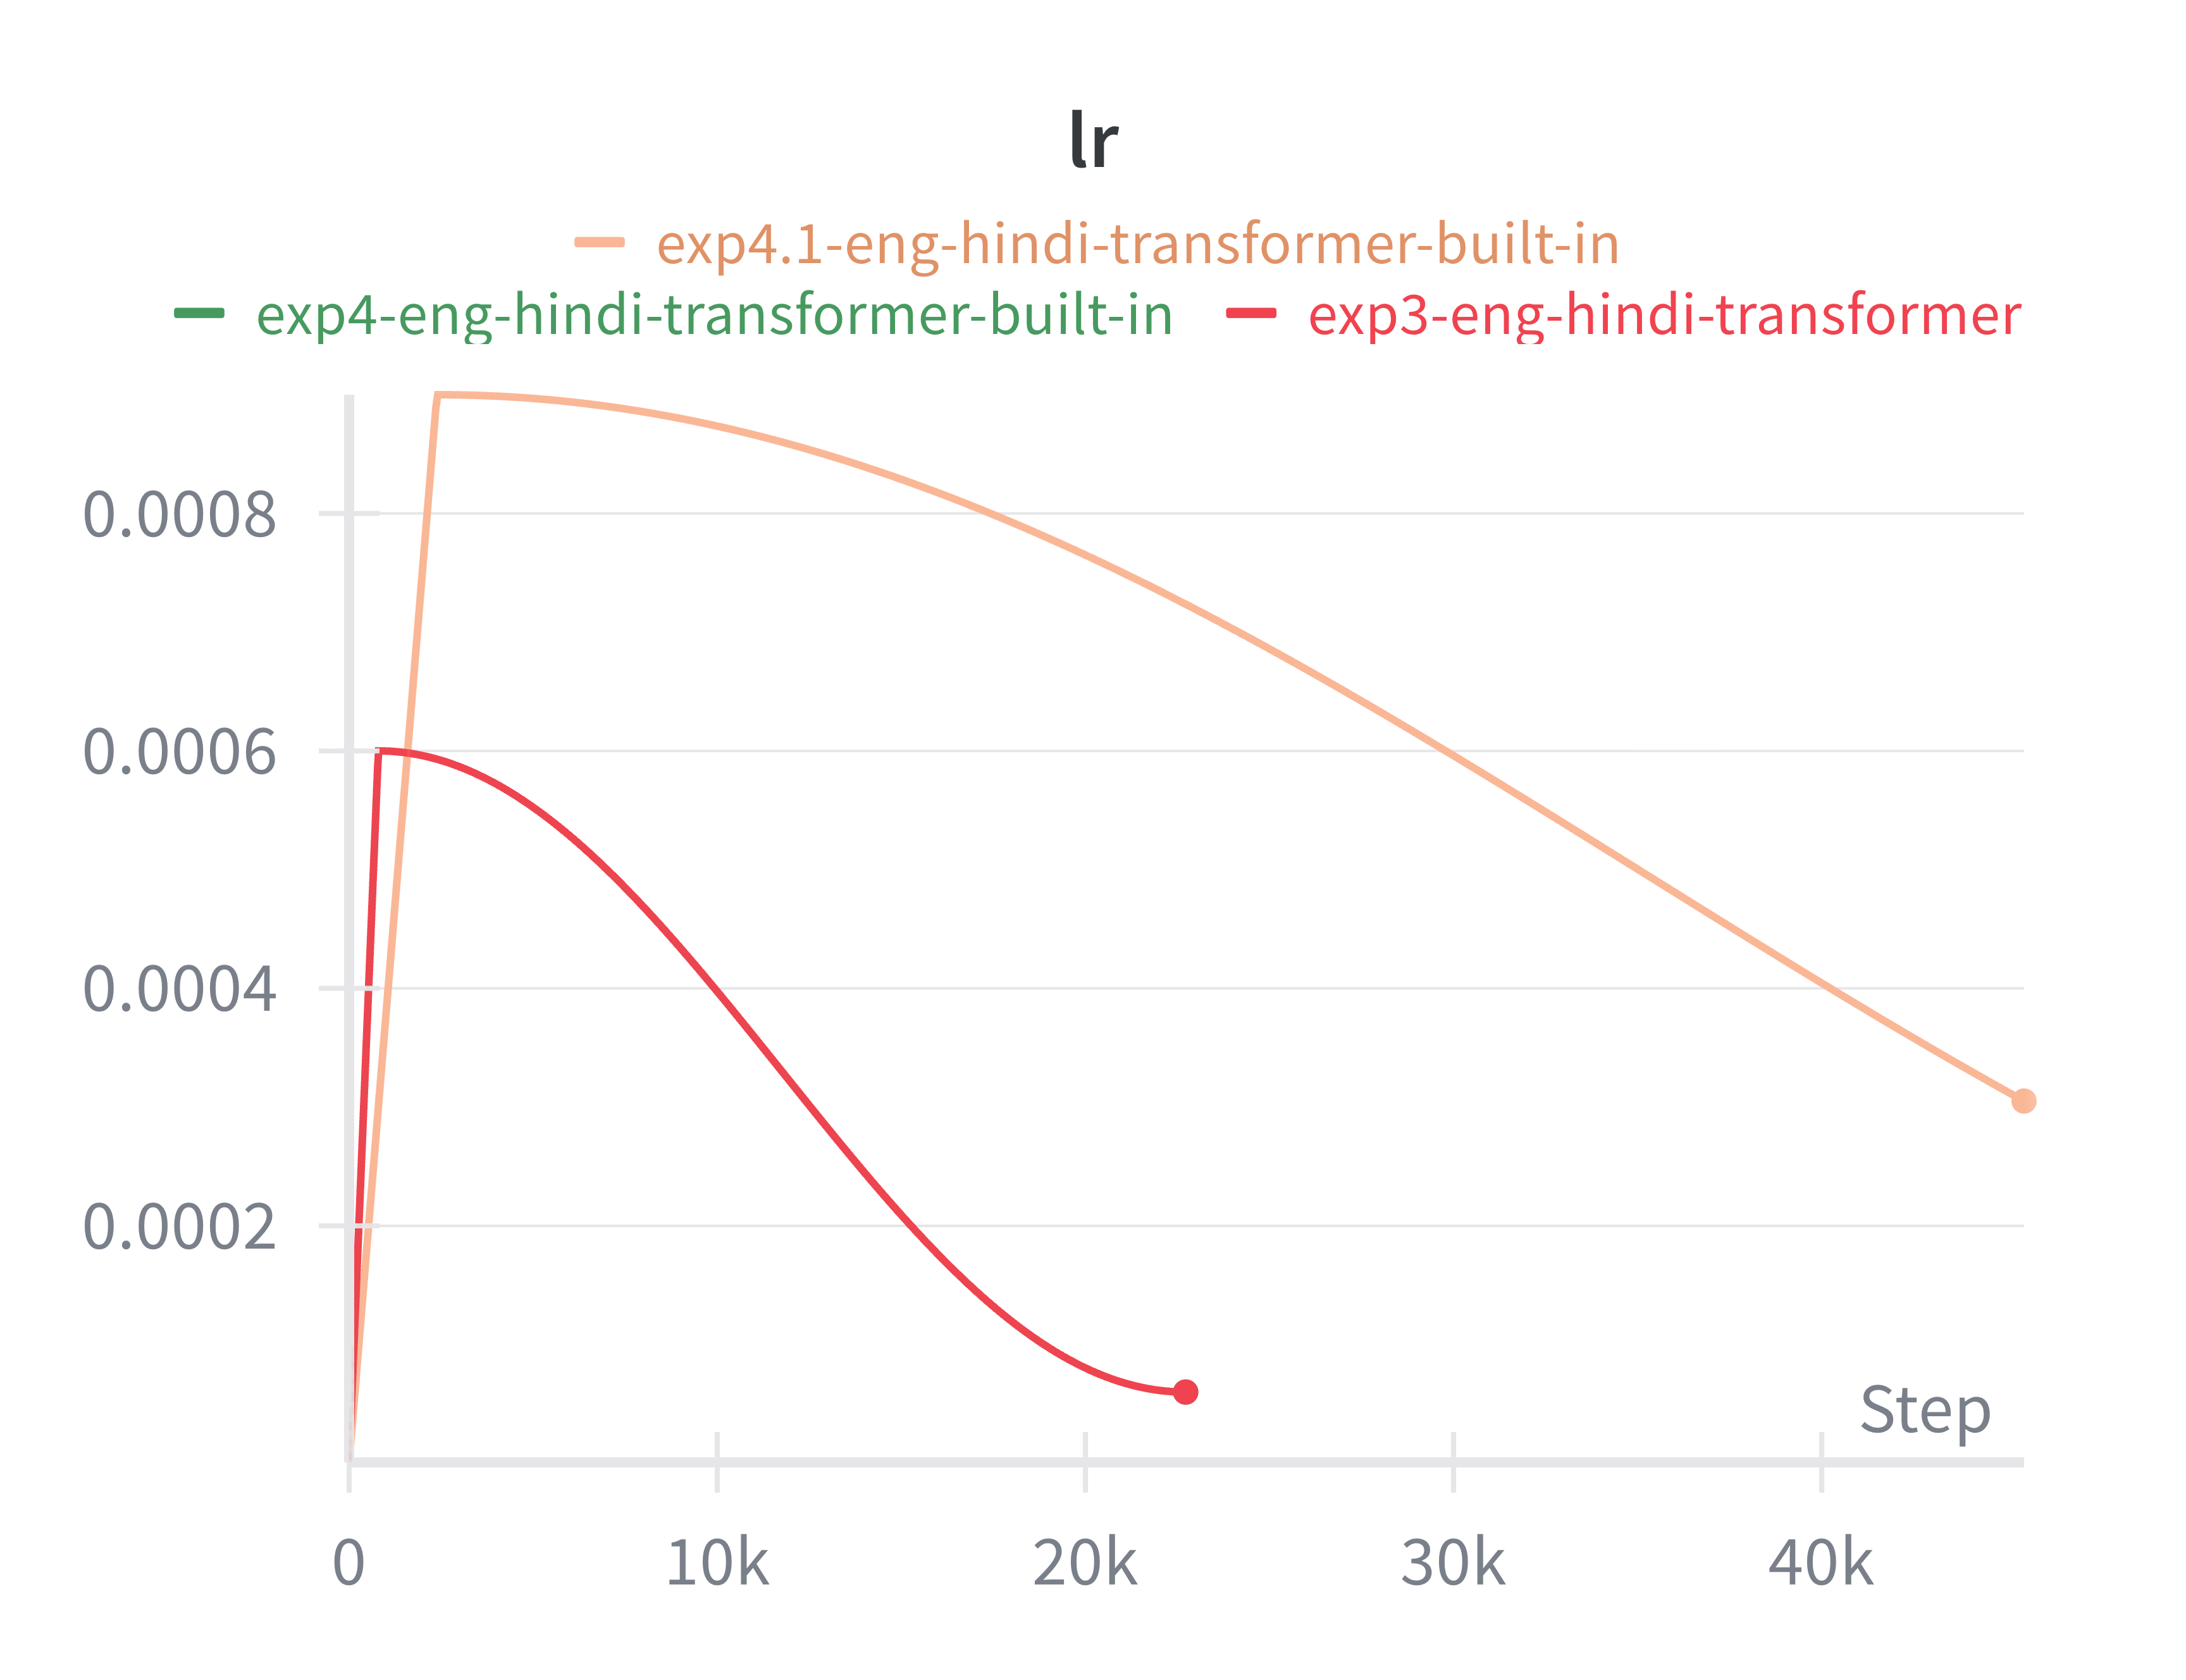
\includegraphics[width=\textwidth]{wandb/lr_hindi.png}
    \caption{Learning rate (Hindi)}
    \label{fig:lr_hindi}
\end{minipage}
\hfill
\begin{minipage}{0.18\textwidth}
    \centering
    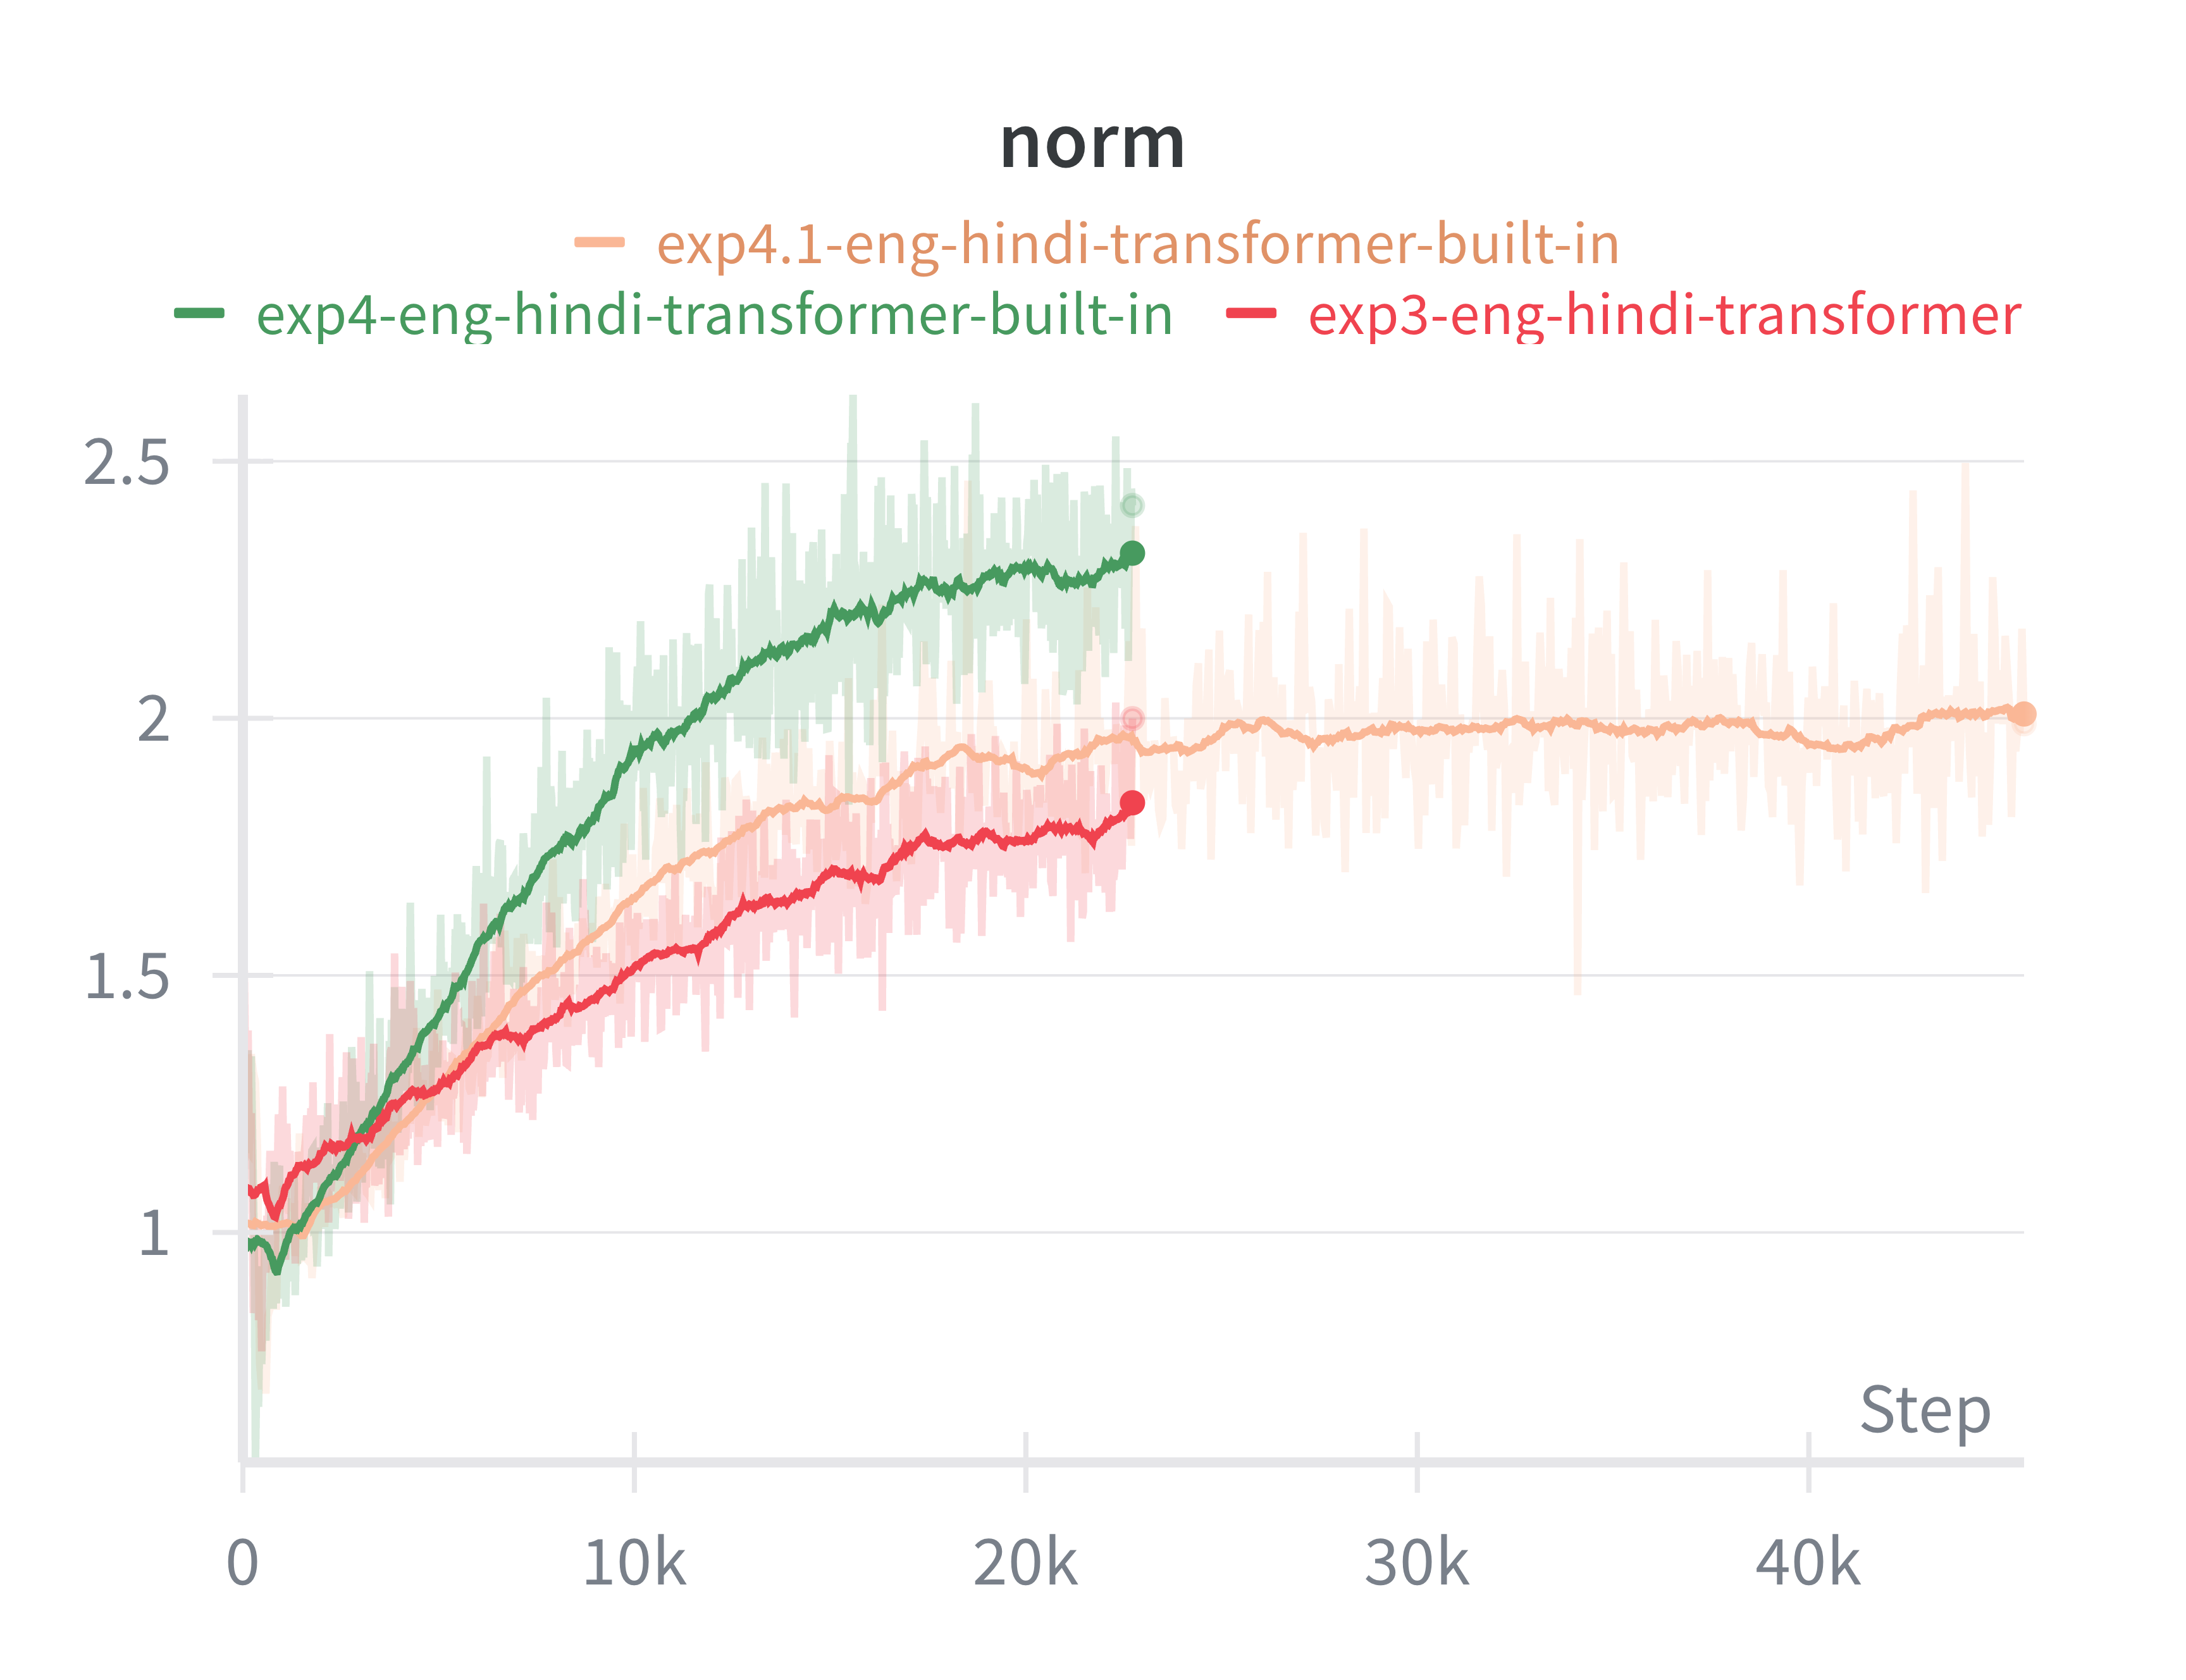
\includegraphics[width=\textwidth]{wandb/grad_clip_hindi.png}
    \caption{Grad norm (Hindi)}
    \label{fig:grad_hindi}
\end{minipage}
\hfill
\begin{minipage}{0.18\textwidth}
    \centering
    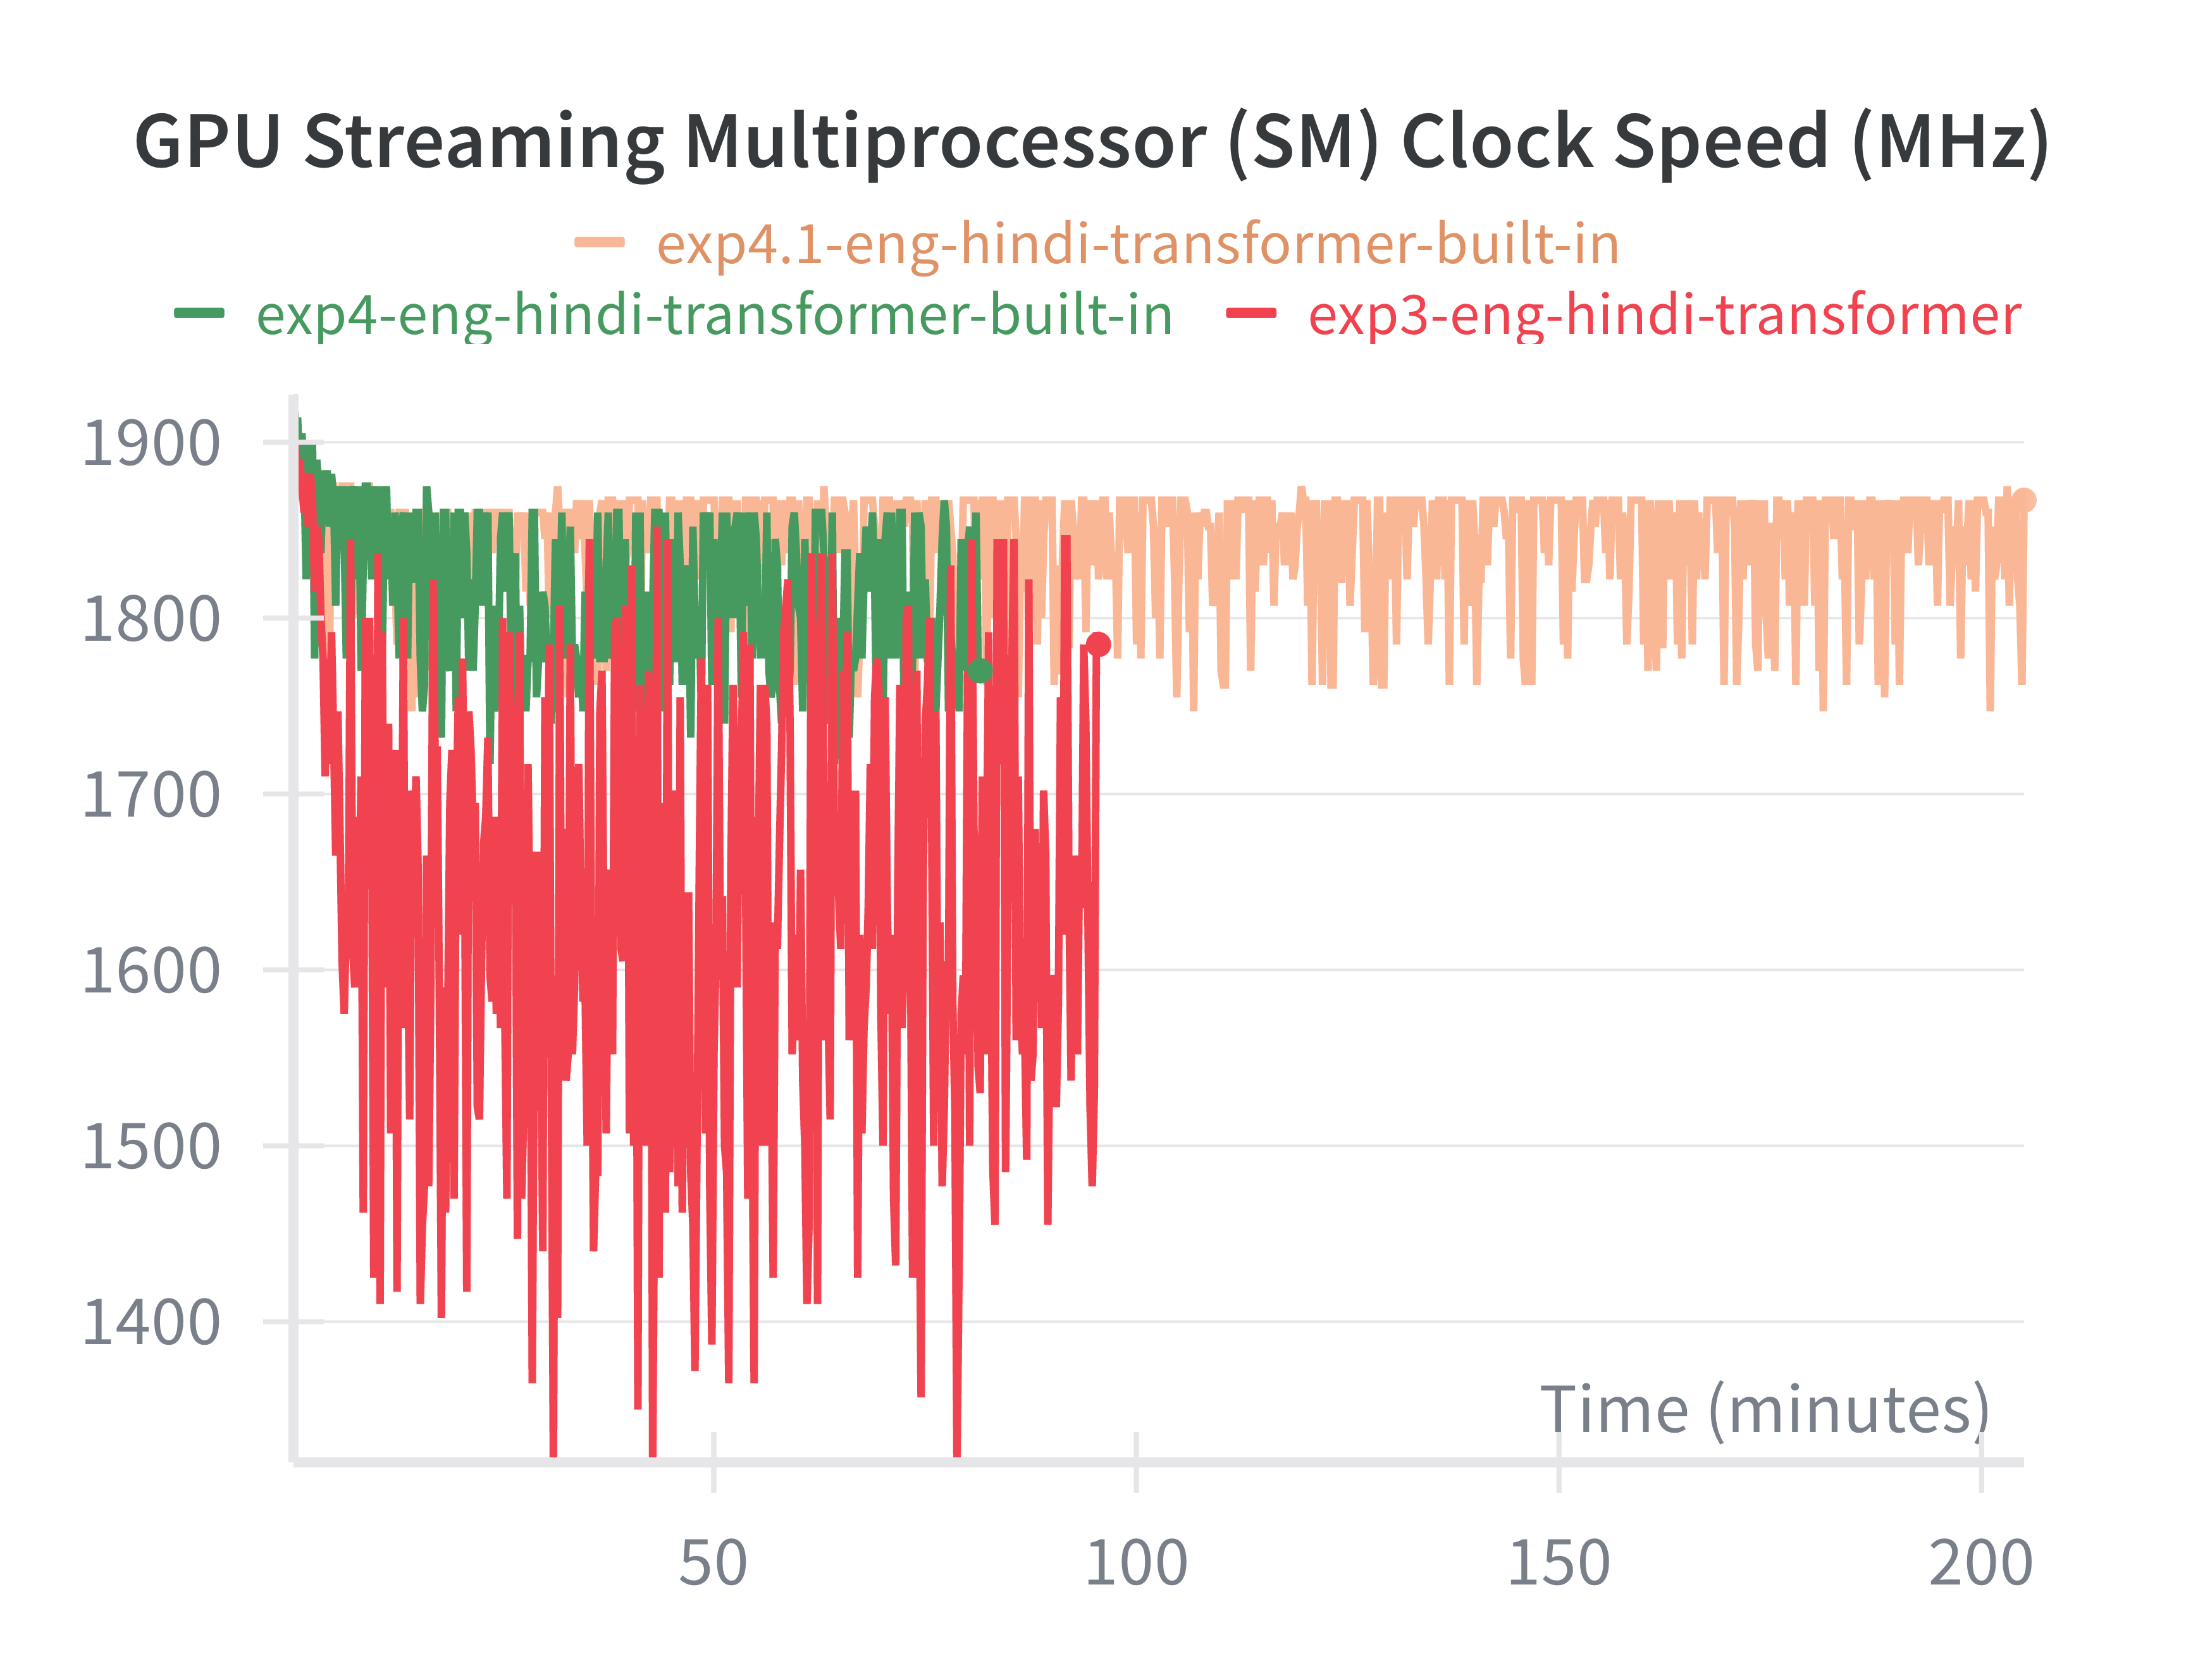
\includegraphics[width=\textwidth]{wandb/gpu_hindi.png}
    \caption{GPU usage (Hindi)}
    \label{fig:gpu_hindi}
\end{minipage}
\end{figure}


\begin{figure}[h]
\centering
\begin{minipage}{0.18\textwidth}
    \centering
    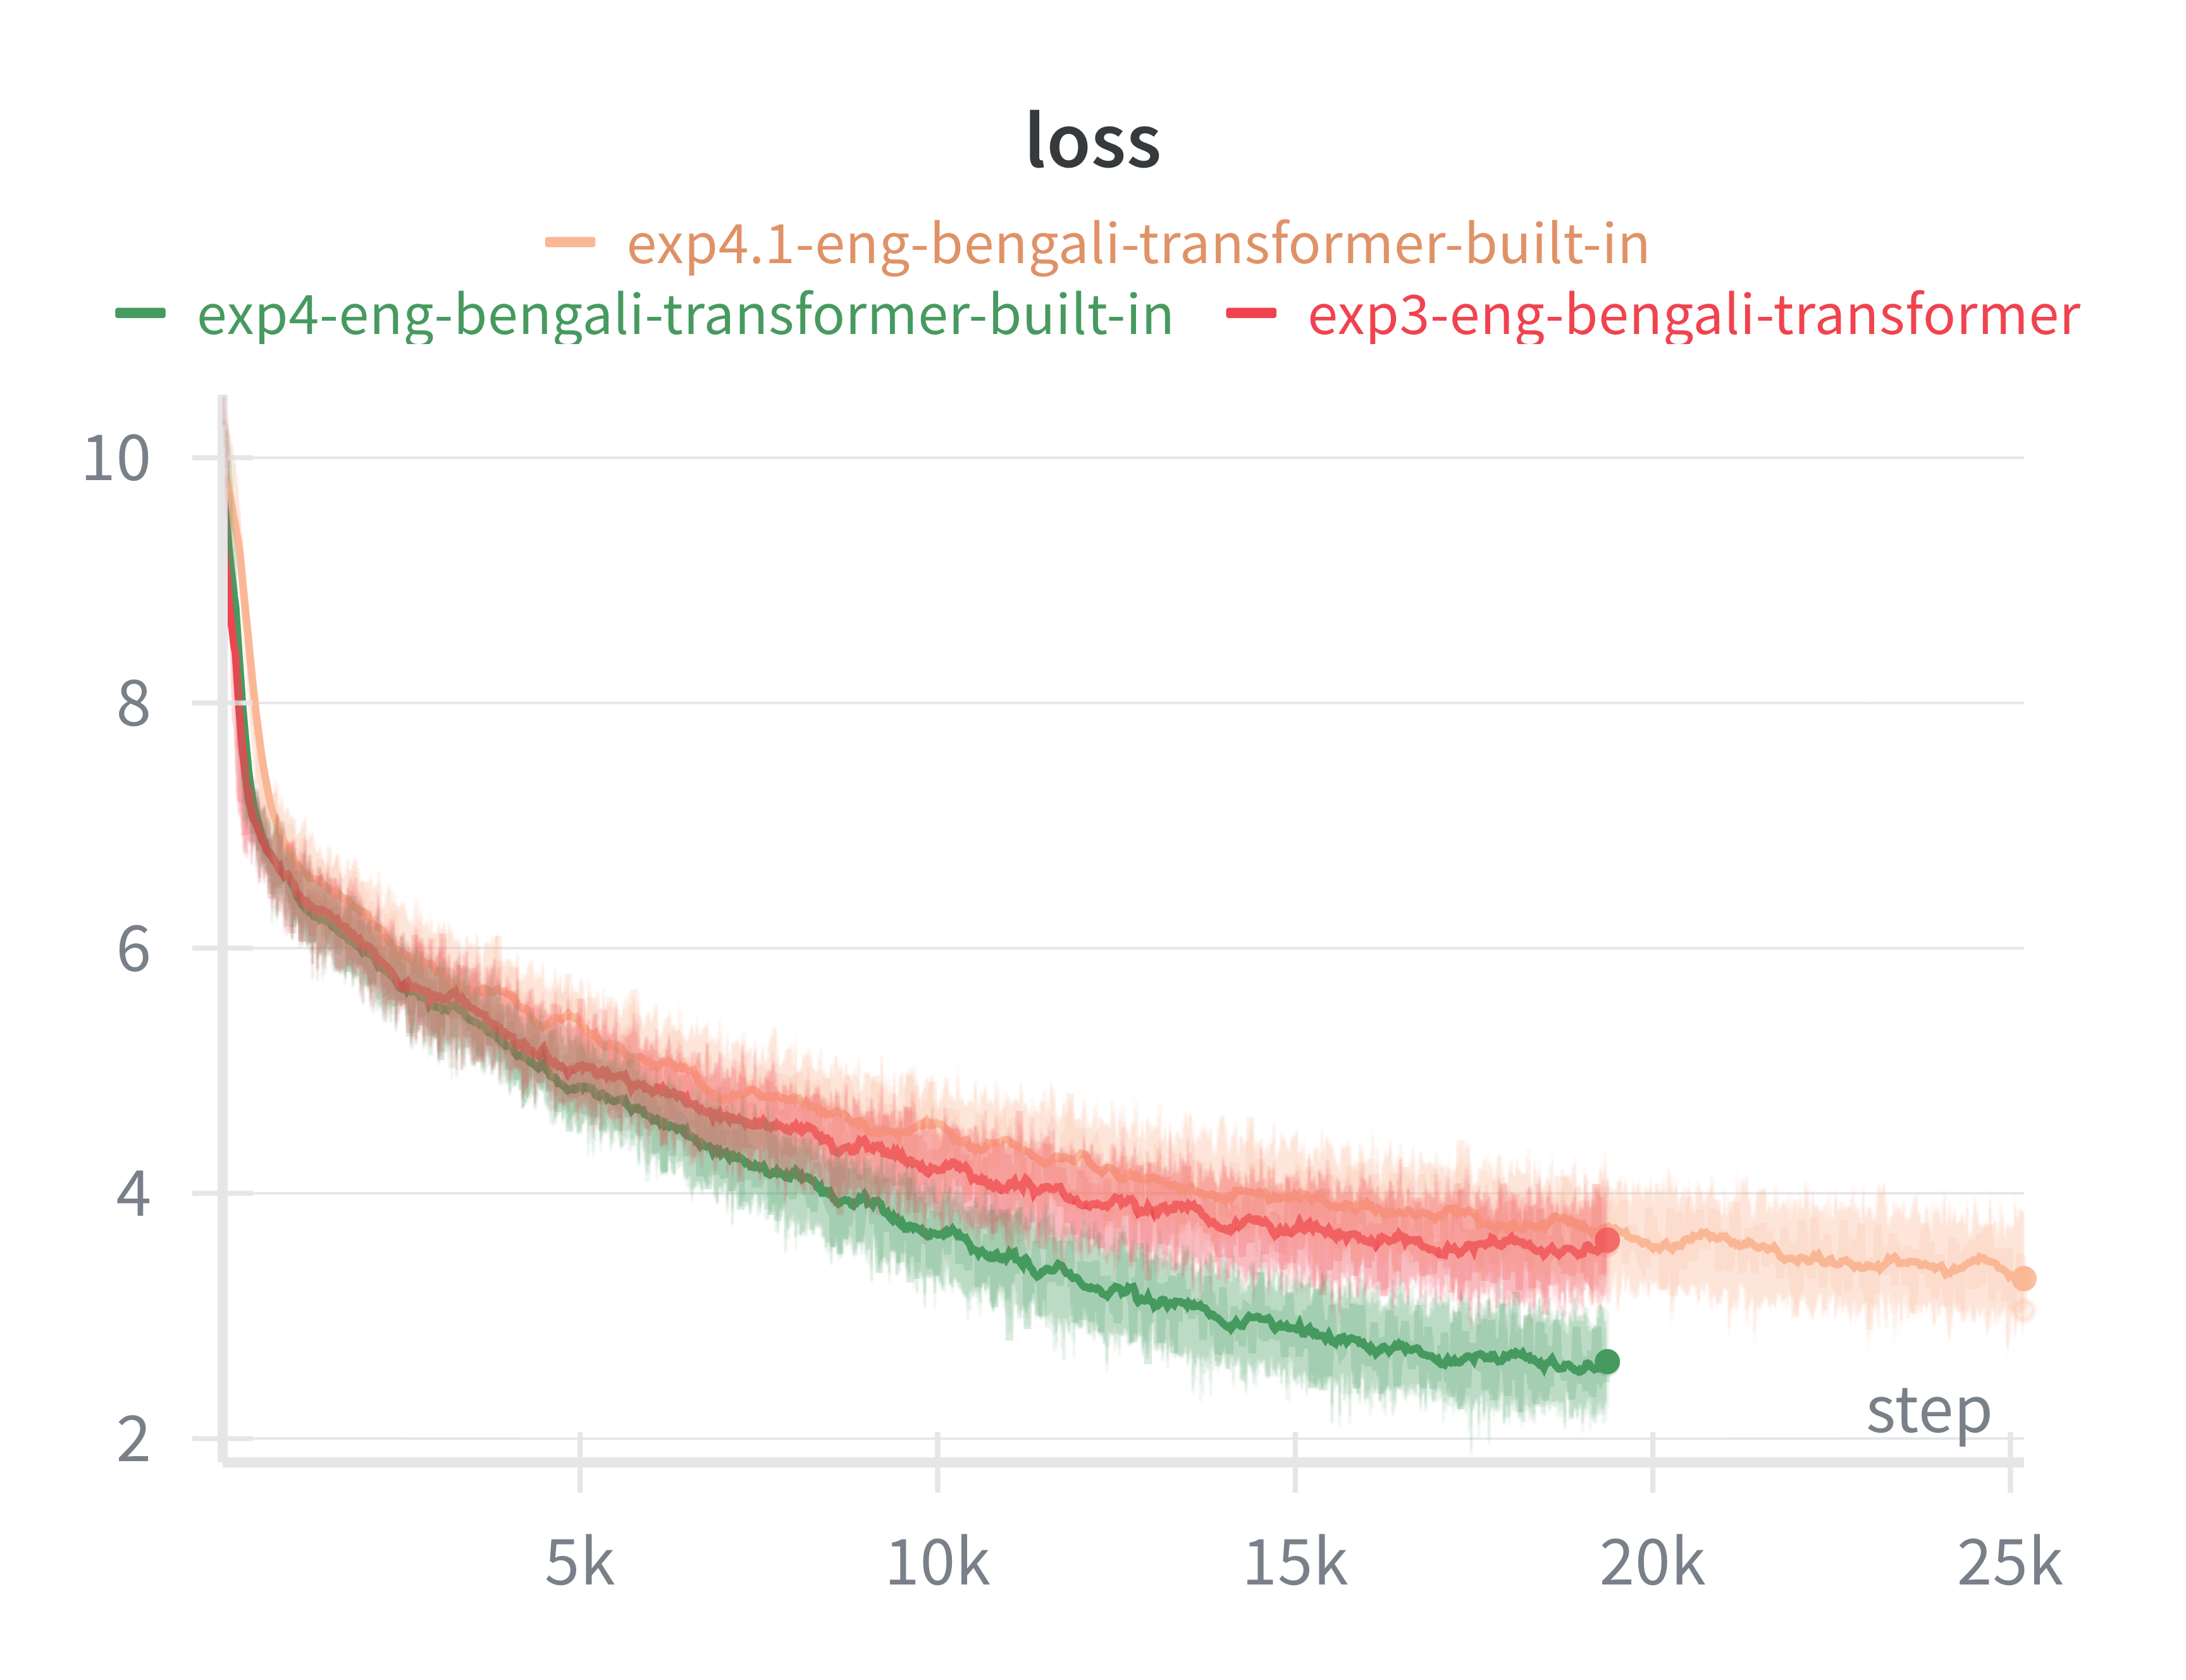
\includegraphics[width=\textwidth]{wandb/cross_entropy_loss_bengali.png}
    \caption{Training loss (Bengali)}
    \label{fig:loss_bengali}
\end{minipage}
\hfill
\begin{minipage}{0.18\textwidth}
    \centering
    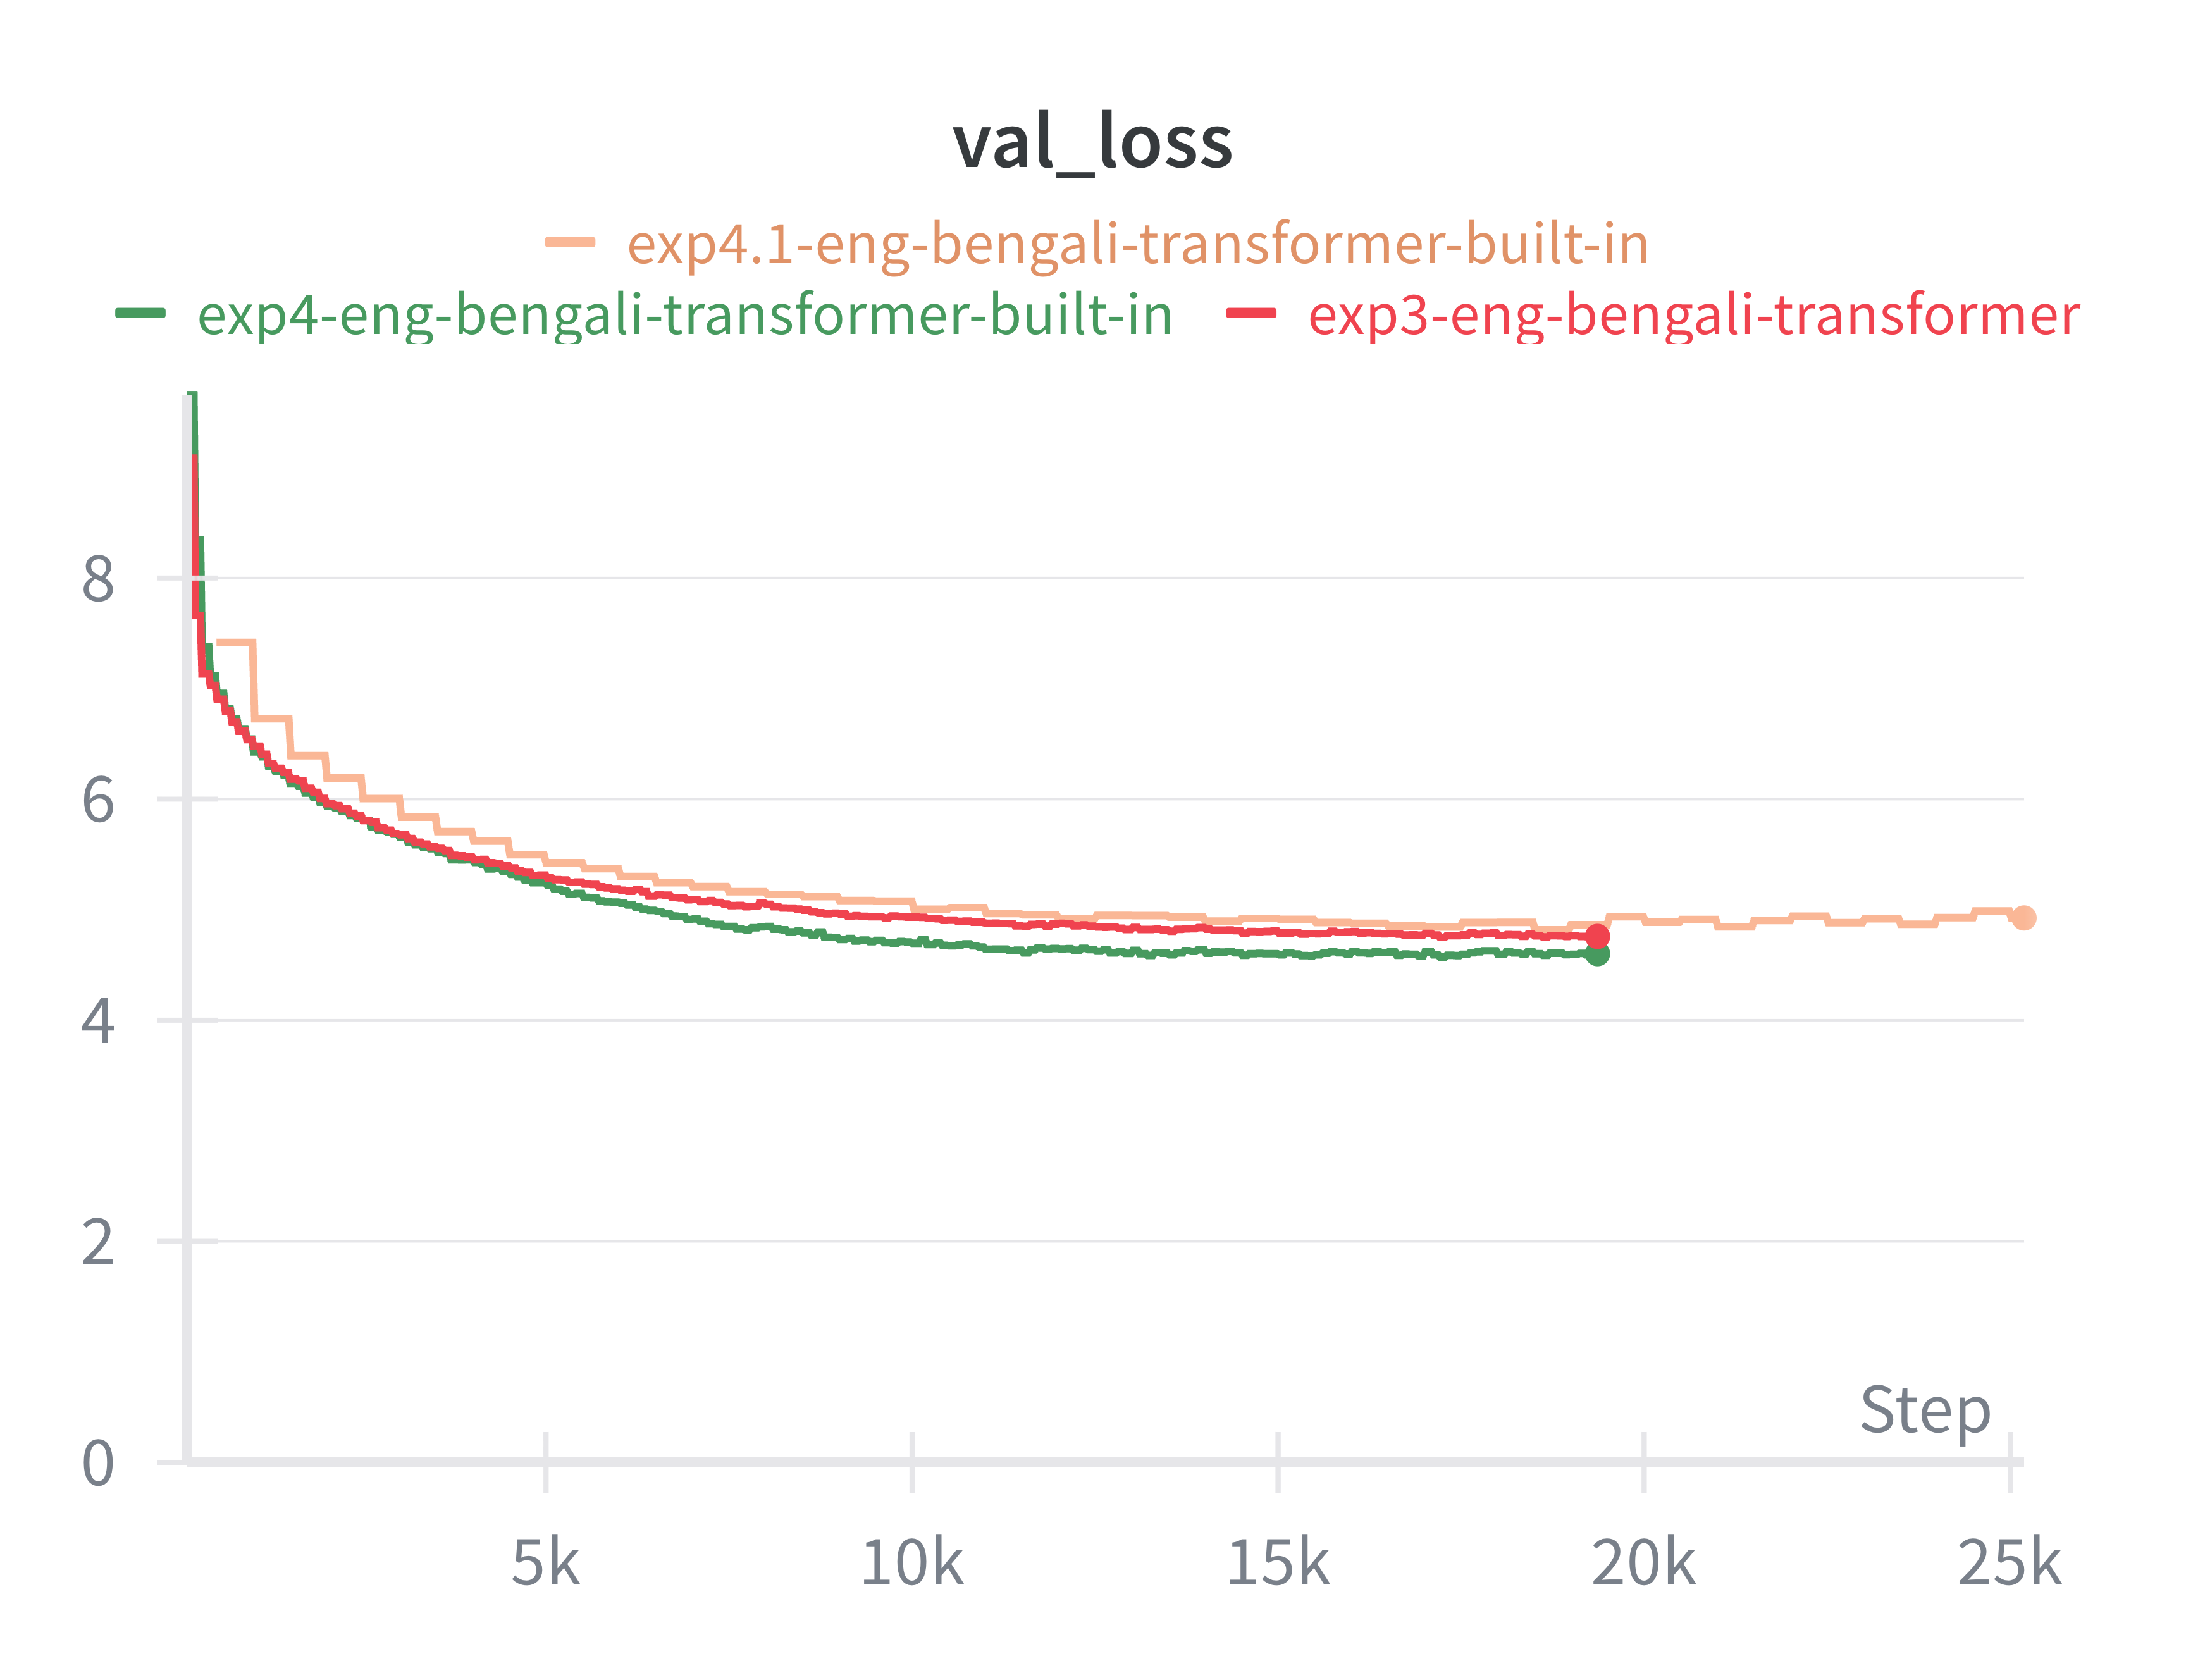
\includegraphics[width=\textwidth]{wandb/val_loss_bengali.png}
    \caption{Validation loss (Bengali)}
    \label{fig:val_loss_bengali}
\end{minipage}
\hfill
\begin{minipage}{0.18\textwidth}
    \centering
    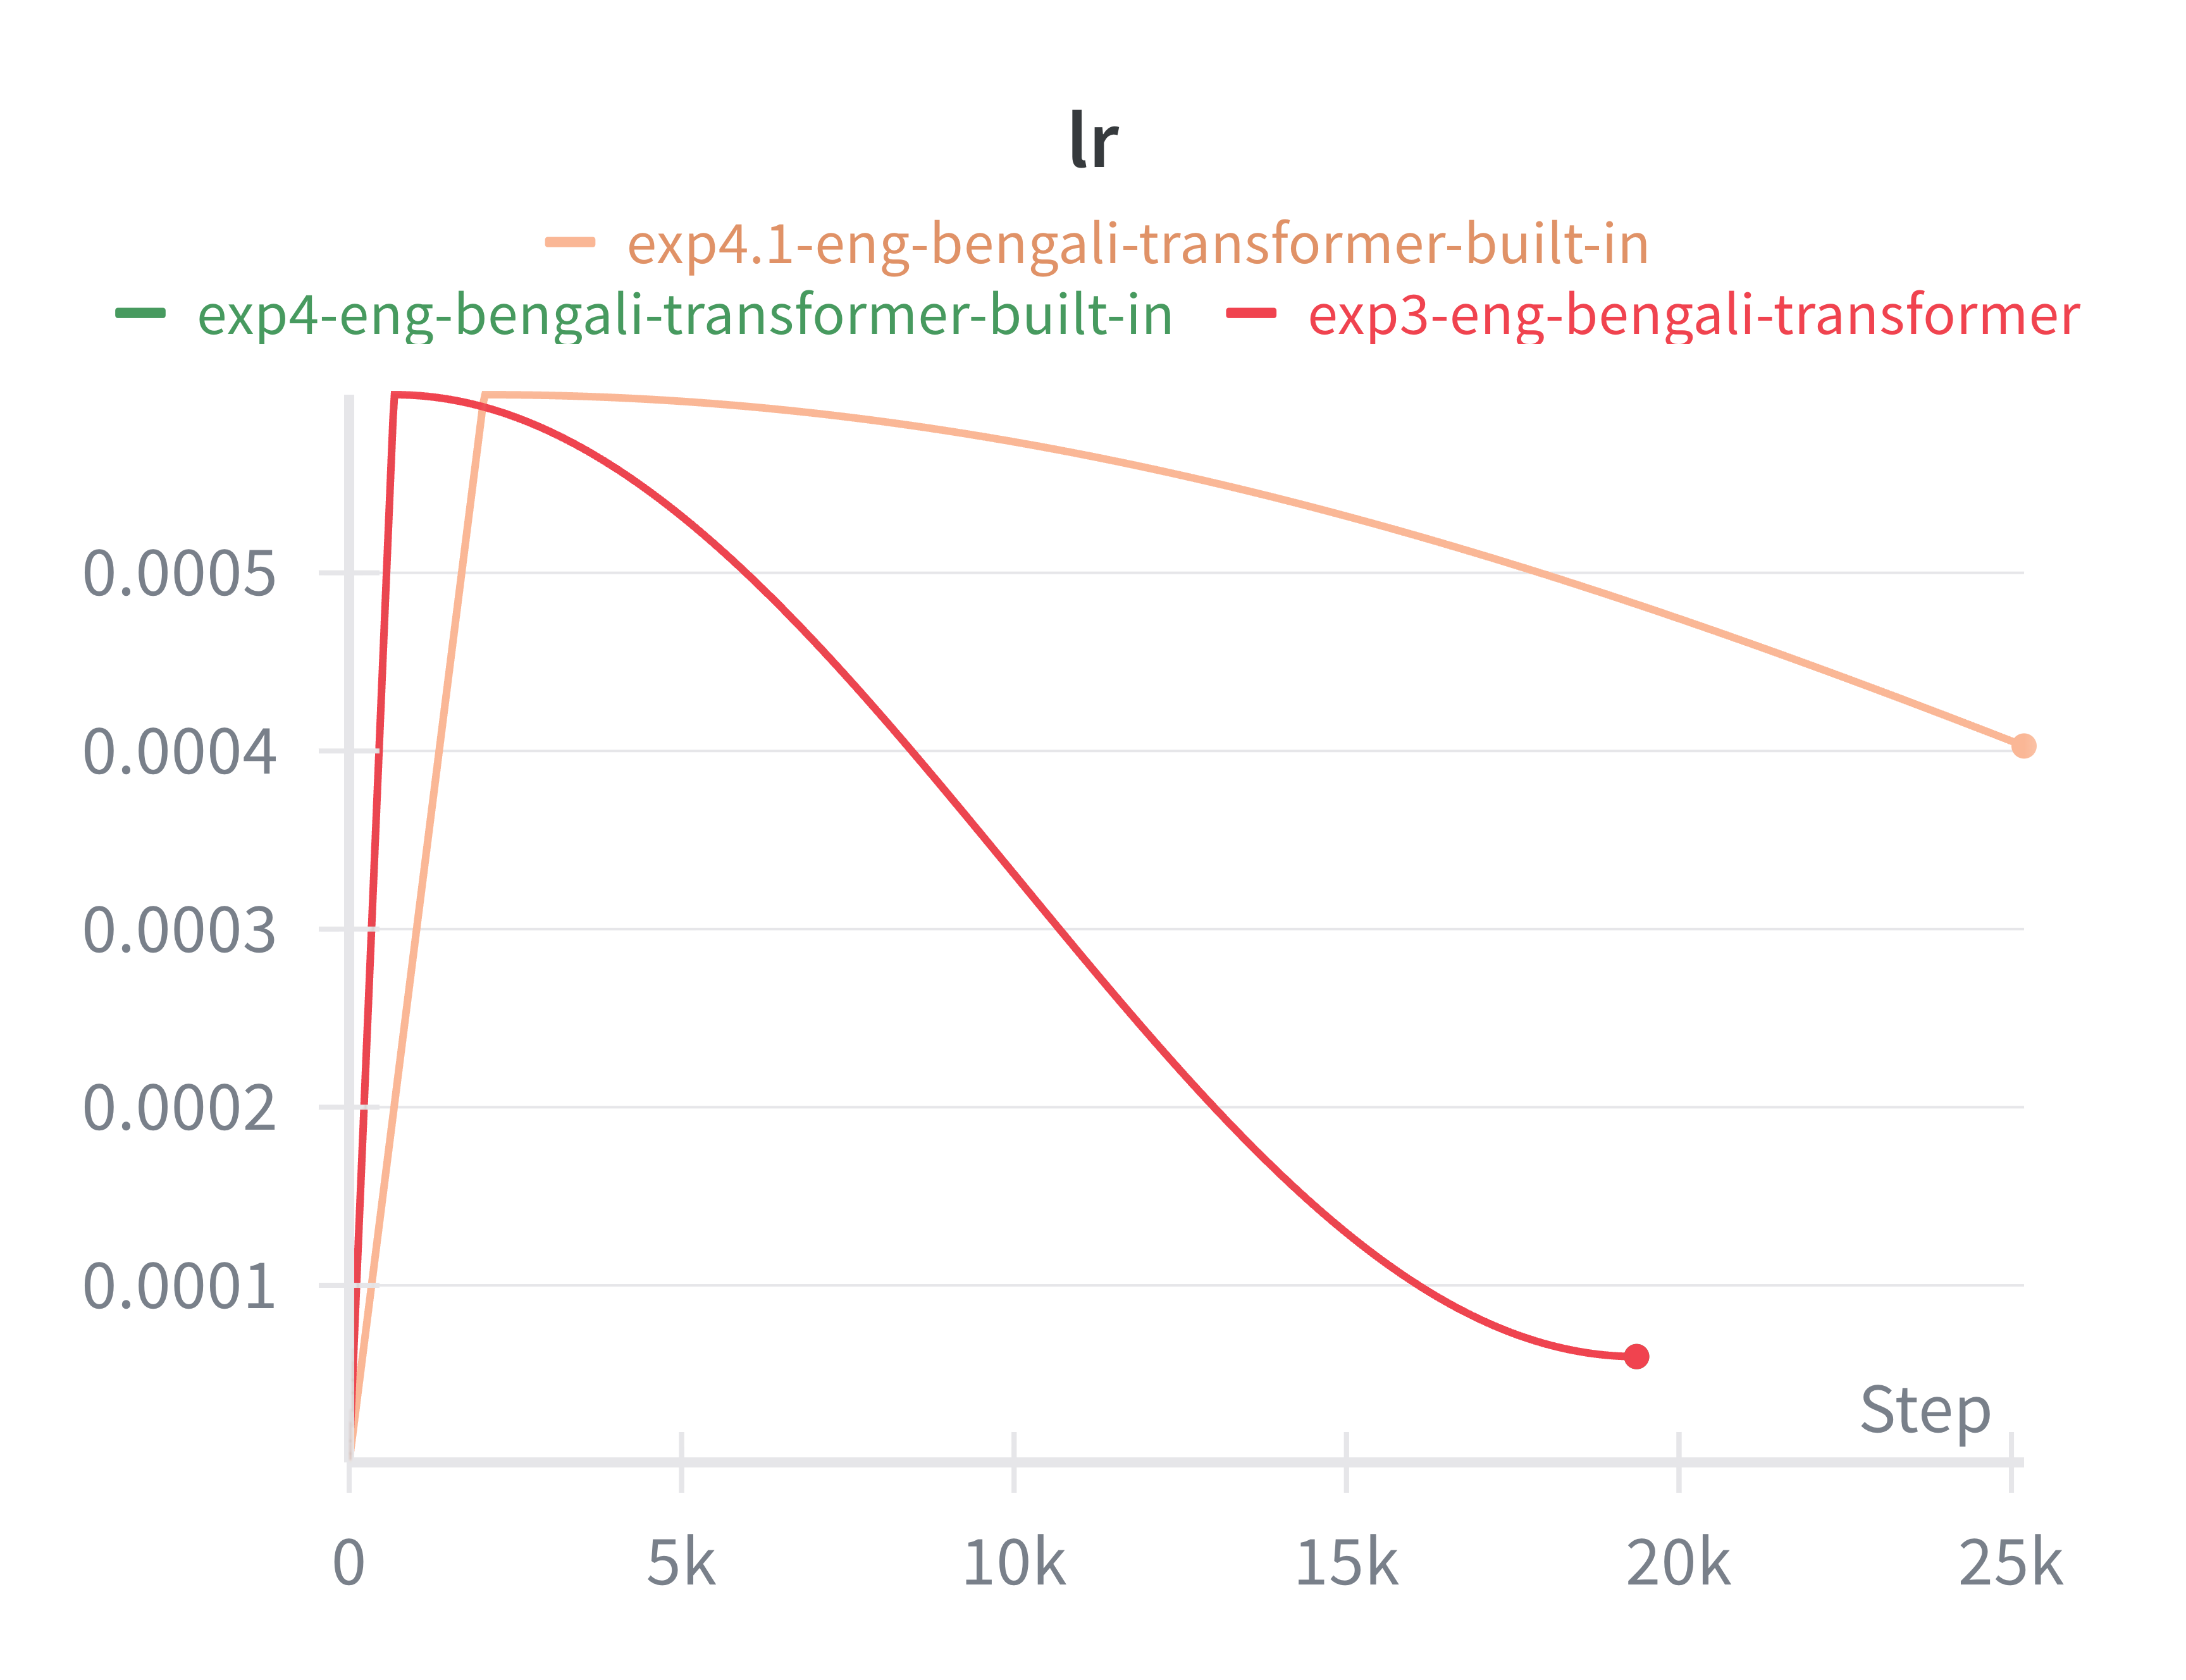
\includegraphics[width=\textwidth]{wandb/lr_bengali.png}
    \caption{Learning rate (Bengali)}
    \label{fig:lr_bengali}
\end{minipage}
\hfill
\begin{minipage}{0.18\textwidth}
    \centering
    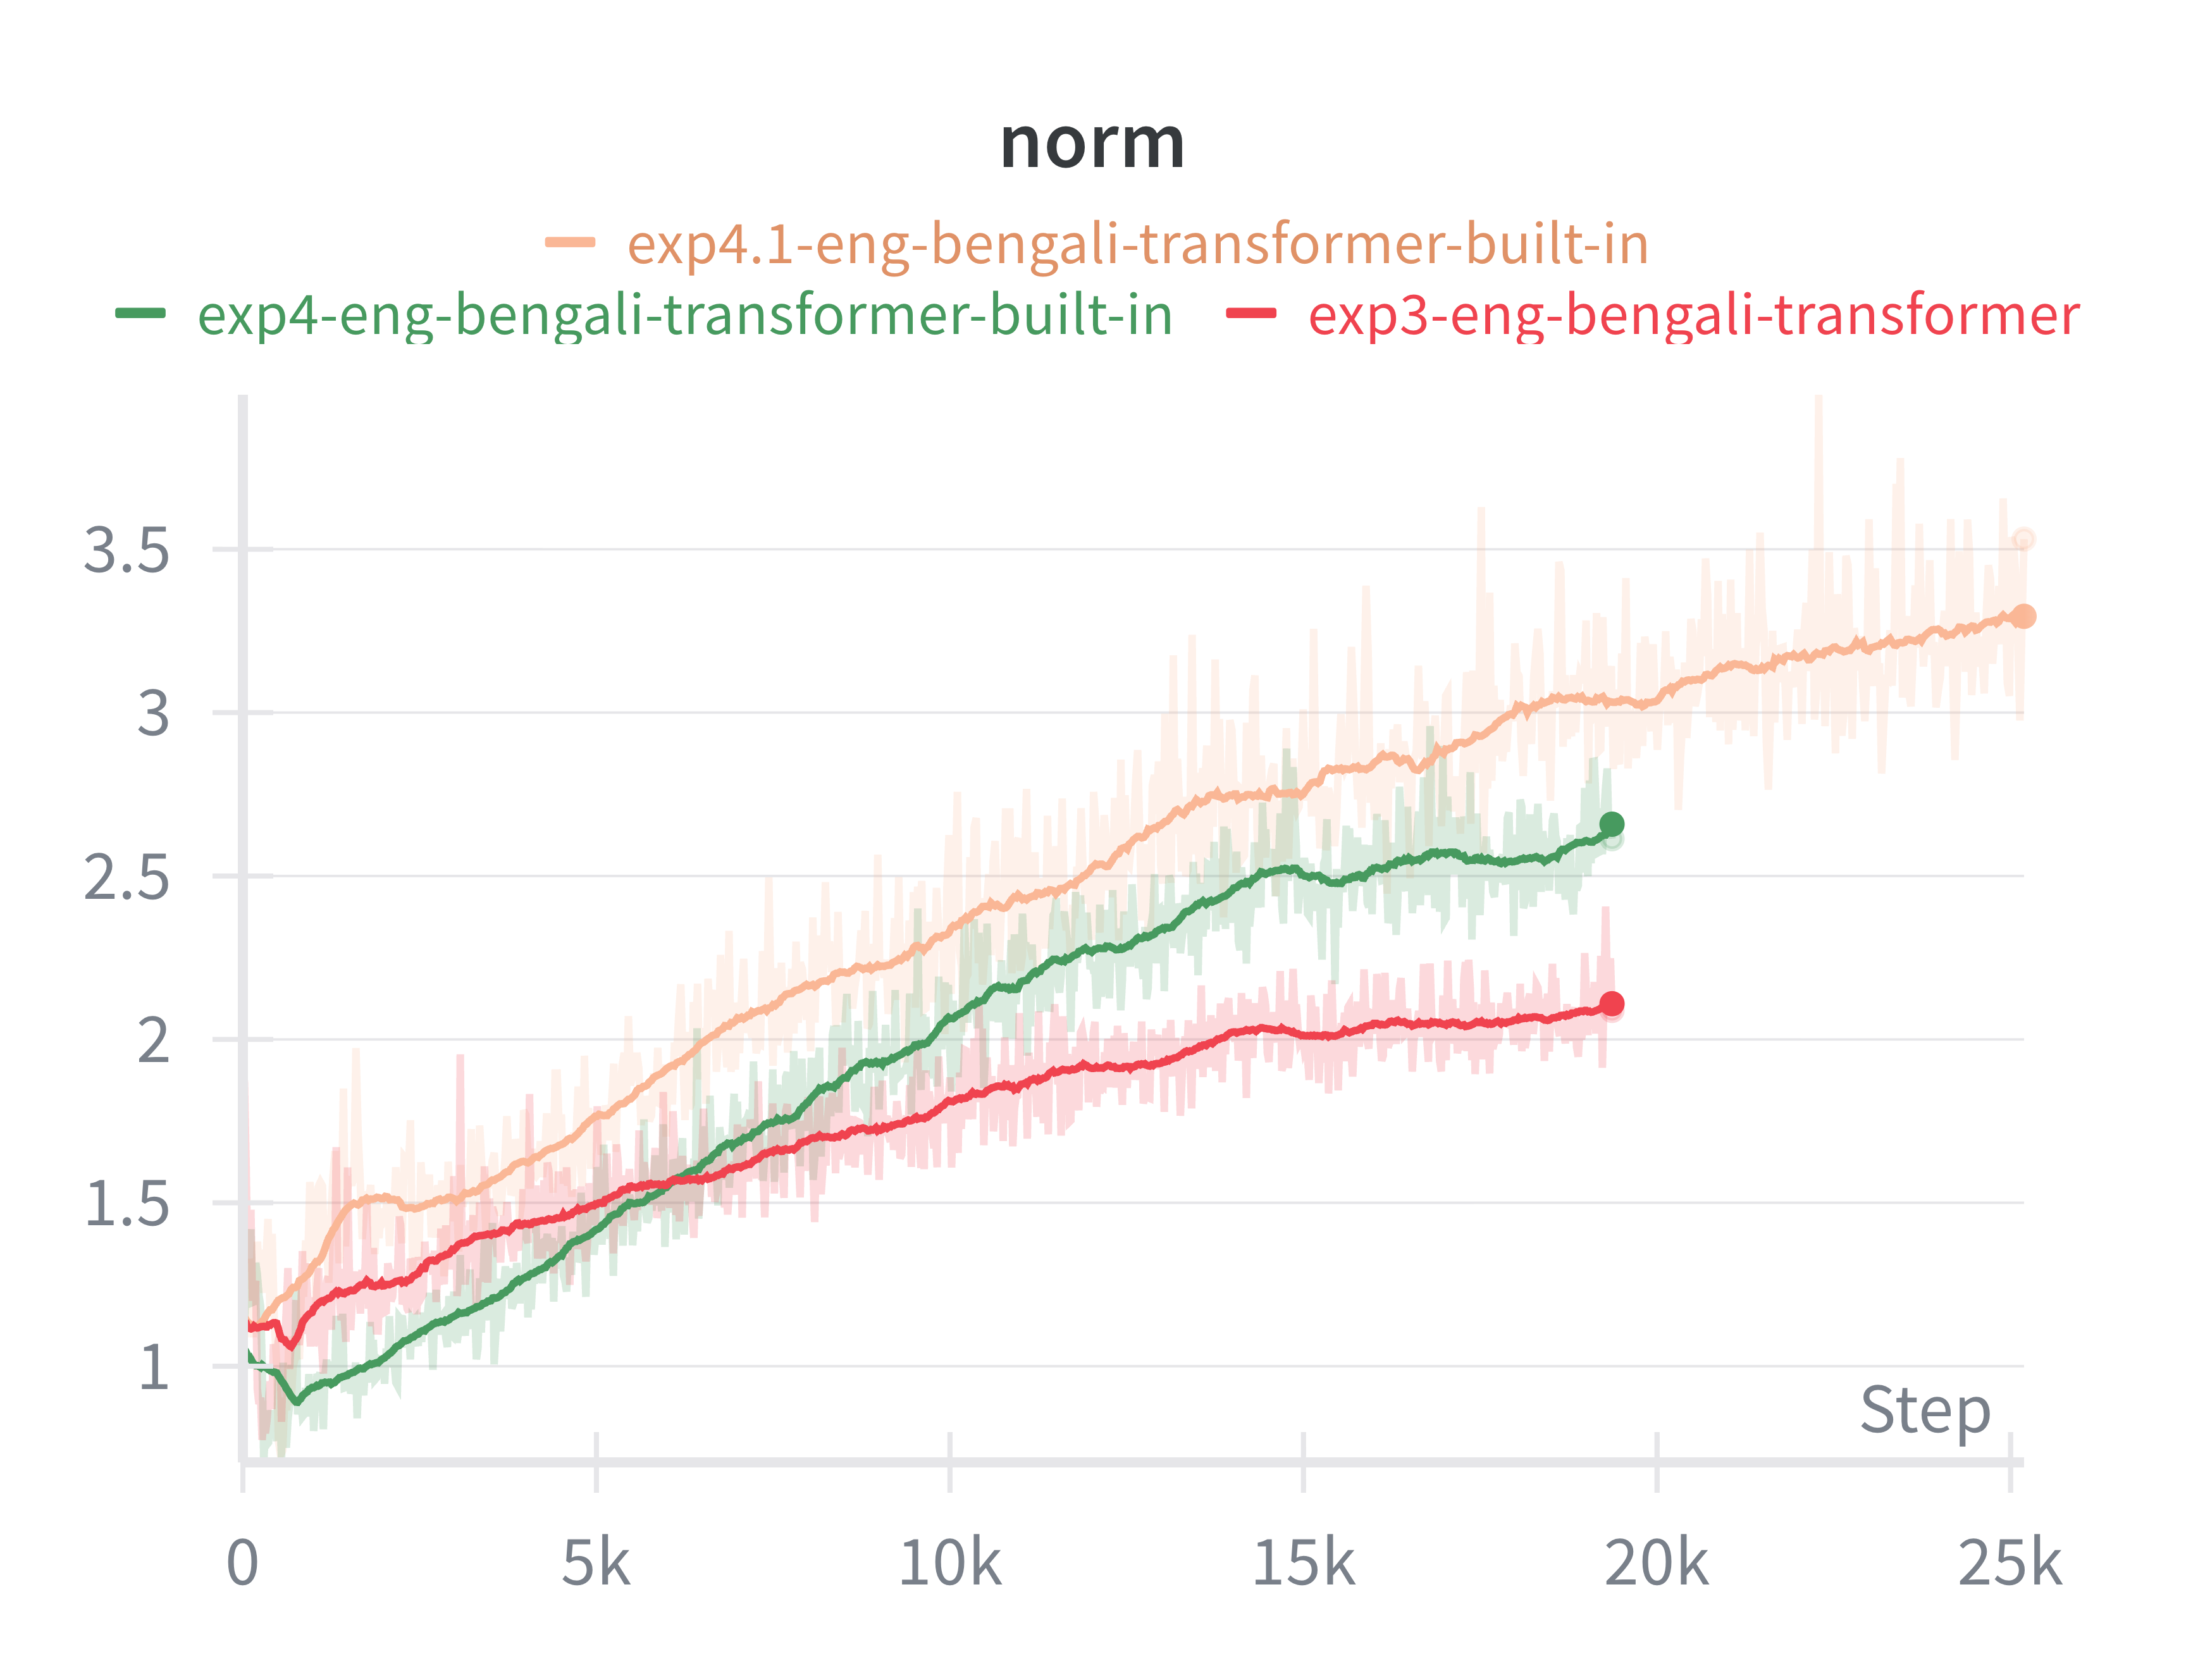
\includegraphics[width=\textwidth]{wandb/grad_clip_bengali.png}
    \caption{Grad norm (Bengali)}
    \label{fig:grad_bengali}
\end{minipage}
\hfill
\begin{minipage}{0.18\textwidth}
    \centering
    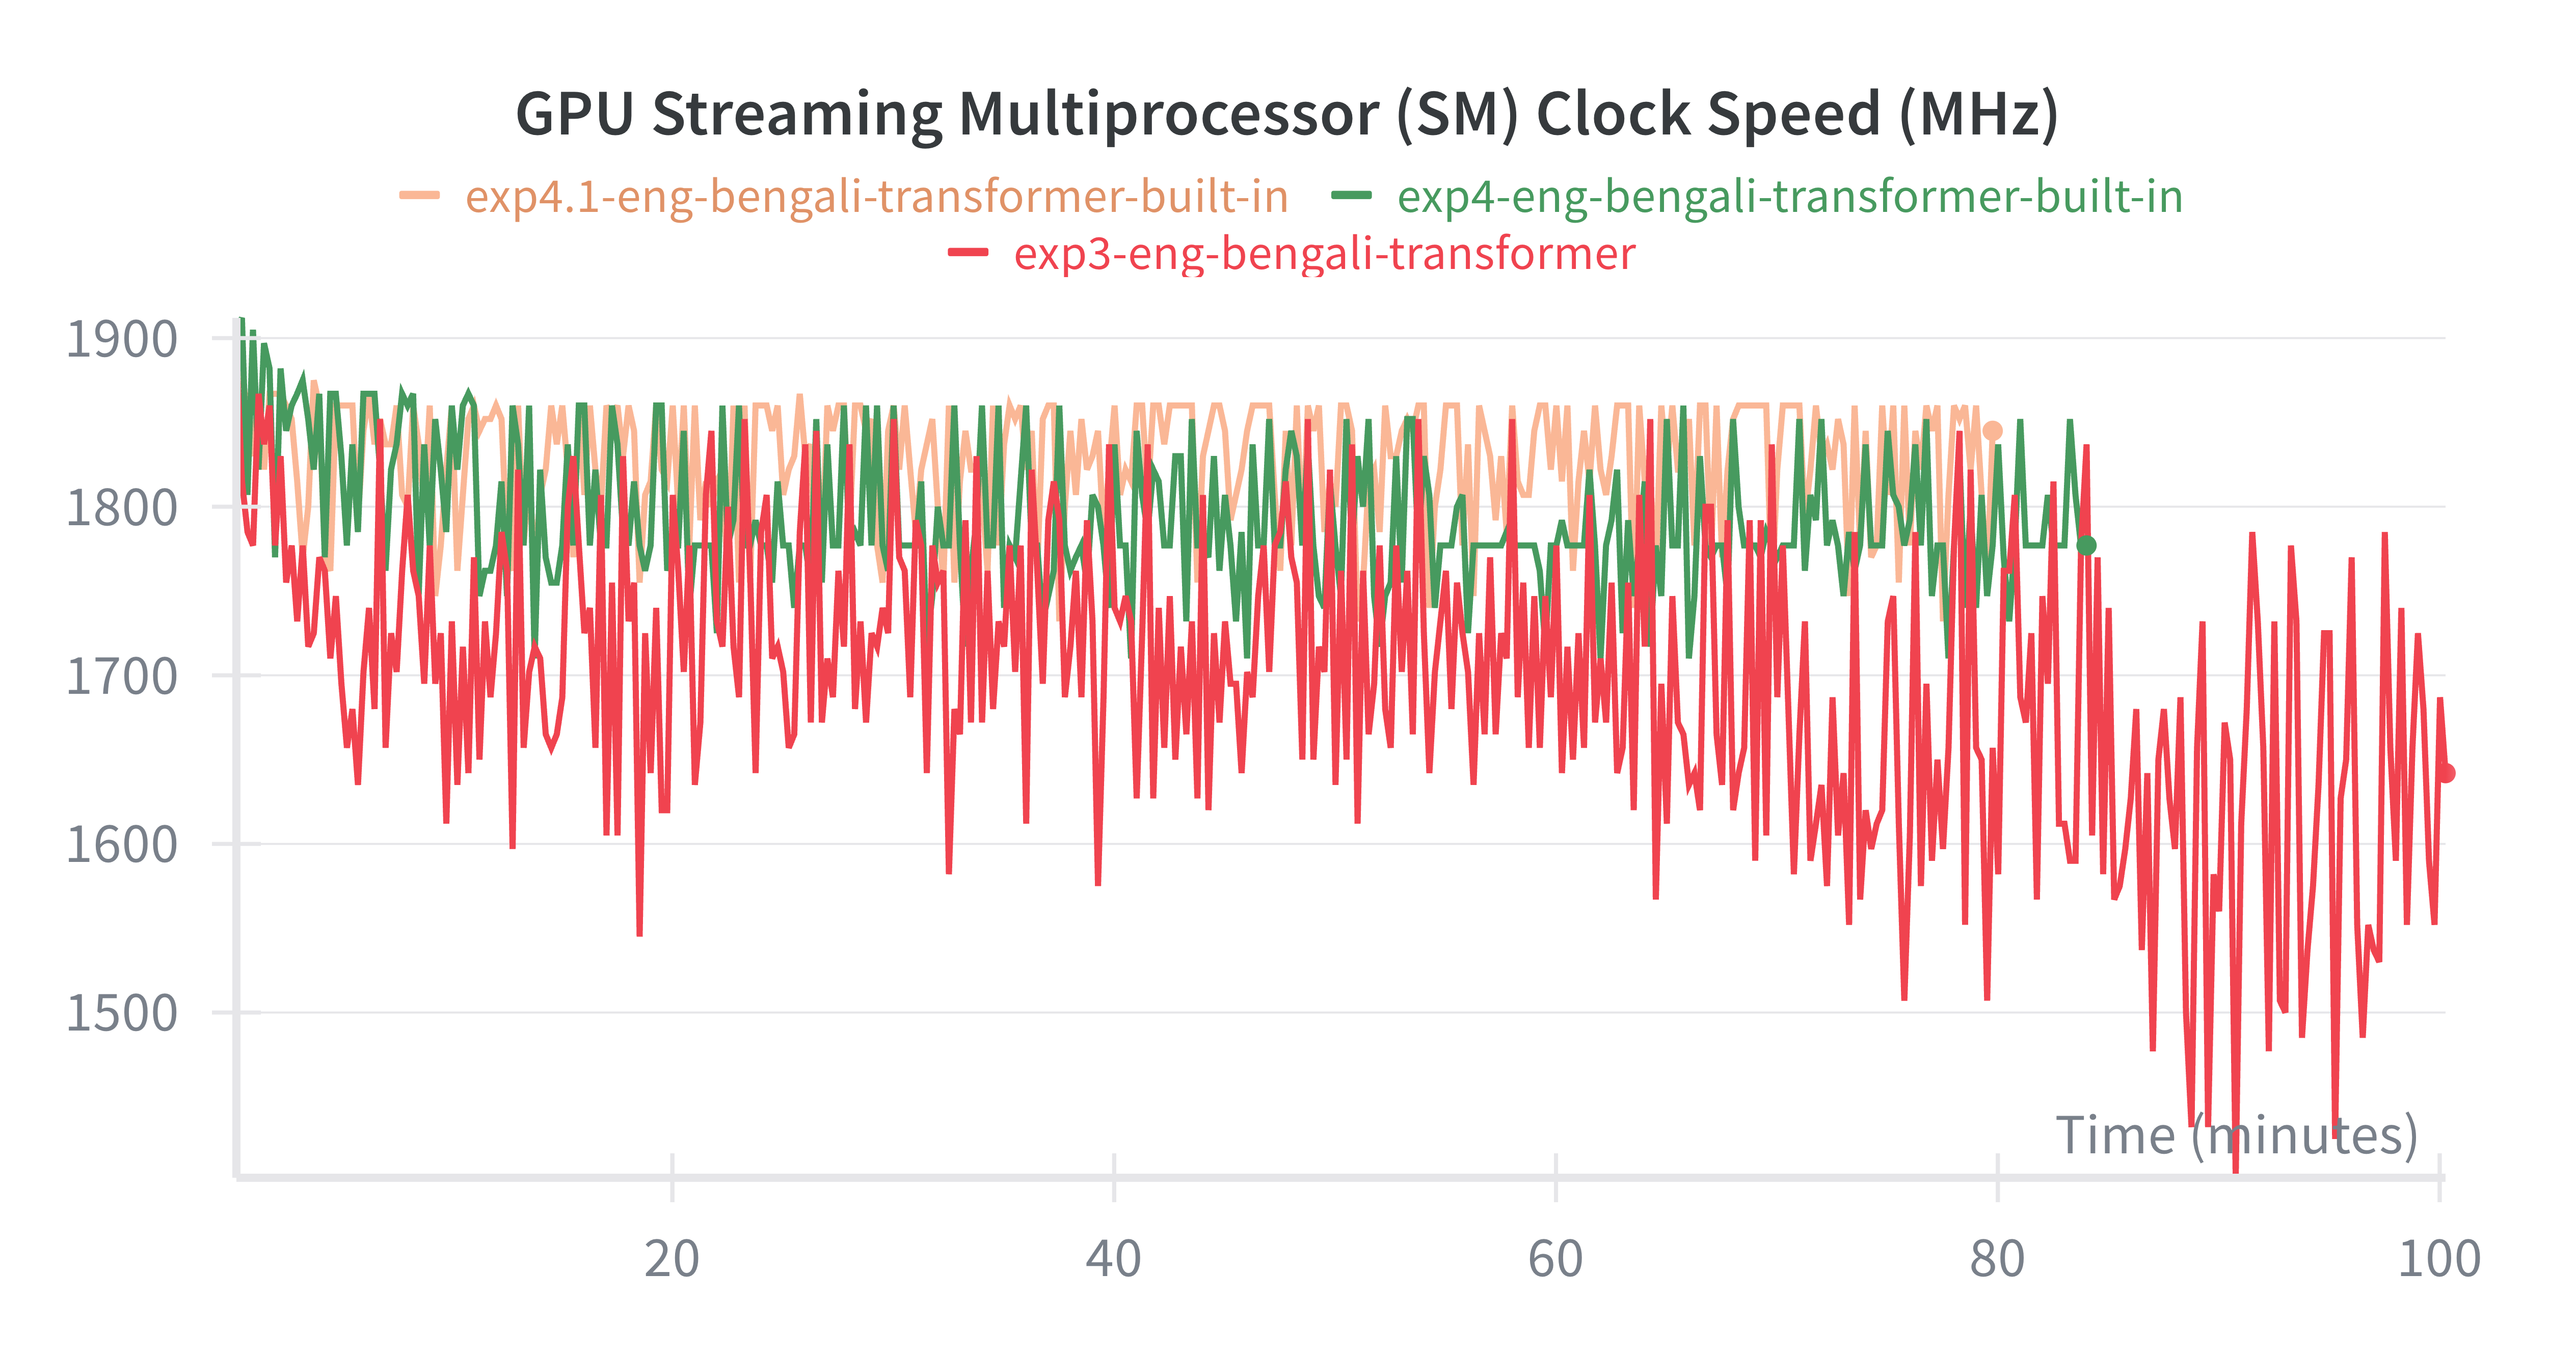
\includegraphics[width=\textwidth]{wandb/gpu_bengali.png}
    \caption{GPU usage (Bengali)}
    \label{fig:gpu_bengali}
\end{minipage}
\end{figure}


Training progress was tracked in Weights \& Biases (wandb) \cite{wandb}, and checkpoints were saved for reproducibility.


% --------------------------------------------------------
% RESULTS
% --------------------------------------------------------
\section{Results}

\subsection{Development Set Performance}
Table~\ref{tab:dev_results} shows results during the train phase. Transitioning from a custom Transformer to PyTorch’s \texttt{nn.Transformer} gave a clear boost across all metrics, and extended training (Experiment~3) achieved the best scores.

\begin{table}[h]
\centering
\caption{Development Set Results}
\label{tab:dev_results}
\begin{tabular}{|l|c|c|c|c|c|}
\hline
\textbf{Experiment} & \textbf{Rank} & \textbf{BLEU} & \textbf{ROUGE} & \textbf{chrF++} & \textbf{Total} \\
\hline
Exp~1 (custom)  & -- & 0.063 & 0.334 & 0.275 & 0.672 \\
Exp~2 (nn.Transf.) & -- & 0.114 & 0.401 & 0.374 & 0.889 \\
Exp~3 (30 epochs) & \#1 & \textbf{0.126} & \textbf{0.410} & \textbf{0.396} & \textbf{0.932} \\
\hline
\end{tabular}
\end{table}

\subsection{Test Set Performance}
On the final leaderboard (Table~\ref{tab:test_results}), Experiment~3 generalized well, securing Rank~\#2 overall with a total score of 0.957.

\begin{table}[h]
\centering
\caption{Test Set Results}
\label{tab:test_results}
\begin{tabular}{|l|c|c|c|c|c|}
\hline
\textbf{Experiment} & \textbf{Rank} & \textbf{BLEU} & \textbf{ROUGE} & \textbf{chrF++} & \textbf{Total} \\
\hline
Exp~1 (custom)  & -- & 0.022 & 0.198 & 0.128 & 0.348 \\
Exp~2 (nn.Transf.) & -- & 0.125 & 0.410 & 0.380 & 0.915 \\
Exp~3 (30 epochs) & \#2 & \textbf{0.140} & \textbf{0.421} & \textbf{0.396} & \textbf{0.957} \\
\hline
\end{tabular}
\end{table}

\subsection{Performance Analysis}
Experiment~3 gave the strongest results: BLEU improved from 0.126 (dev) to 0.140 (test), showing good generalization.  
Key factors behind this improvement were:  
\begin{itemize}
    \item Switching from a custom to PyTorch’s optimized \texttt{nn.Transformer}, which improved stability and efficiency.  
    \item Longer training (30 epochs) with tuned learning rates and more attention heads for Hindi (8 vs.\ 4).  
    \item Cosine LR scheduling with warmup, which stabilized convergence.  
\end{itemize}
Overall, the final model balanced efficiency with performance, ranking \#2 on the leaderboard while avoiding severe overfitting.


% --------------------------------------------------------
% ERROR ANALYSIS
% --------------------------------------------------------
\section{Error Analysis}

\begin{enumerate}
\item \textbf{Implementation Stability:} The custom Transformer was prone to numerical instability and poor GPU utilization, which limited training efficiency. In contrast, PyTorch’s optimized \texttt{nn.Transformer} provided stable training and a large improvement in scores.  

\item \textbf{Training Convergence:} Extended training (30 epochs) improved results, but gradient norms tended to grow rather than stabilize, raising concerns about long-term stability. Validation loss curves also showed overfitting in Experiment~3, indicating the need for stronger regularization or early stopping.  

\item \textbf{Translation Quality:} Despite overall progress, BLEU scores remained low. Errors were most visible in word order, morphology (especially Hindi), and handling of proper nouns. The model sometimes produced fluent but semantically off-target translations, reflecting limitations of word-level tokenization.  

\item \textbf{Key Takeaway:} Implementation quality and training stability had greater impact on performance than architectural tweaks. Addressing overfitting and improving tokenization remain open challenges.  
\end{enumerate}

% --------------------------------------------------------
% CONCLUSION
% --------------------------------------------------------
\section{Conclusion}

This project achieved Rank~\#2 in the competition with BLEU~0.14, chrF++~0.40, and ROUGE~0.42. The strongest gains came from using PyTorch’s \texttt{nn.Transformer}, extending training, and tuning hyperparameters for each task.  

At the same time, the experiments showed that Indic MT remains difficult: word-level vocabularies struggled with morphology and rare words, and models tended to overfit despite careful scheduling.  

\textbf{Future directions:}  
\begin{itemize}
    \item Future improvements could include completing the partially implemented BPE/SentencePiece tokenizers \cite{sennrich2016neural,kudo2018sentencepiece}, data augmentation, incorporating additional corpora, and experimenting with decoder-only GPT-style models \cite{radford2019language,brown2020language}.
    \item Scaling model size and adding regularization methods (e.g., dropout scheduling, label smoothing) to address overfitting.  
\end{itemize}

Overall, the results demonstrate that with careful engineering, even modest Transformer models can perform competitively in low-resource Indic translation. Future work along these lines could push performance further while deepening understanding of architecture–data trade-offs.


\bibliography{references} 
\bibliographystyle{ieeetr}





\end{document}
